% ============================================================
%  ENIAD PFA REPORT — main.tex
%  SafeDrone: Implémentation d'un Modèle Edge-AI pour la
%  Détection de Zones d'Atterrissage Sécurisées
% ============================================================

\documentclass[12pt, a4paper, oneside]{report}

% ── Encodage et langue ──────────────────────────────────────
\usepackage{fontspec}
\usepackage[english, french]{babel}
\babelprovide[import]{arabic}
\babelfont[arabic]{rm}{Arial}
\usepackage{csquotes}

% ── Polices ─────────────────────────────────────────────────
\usepackage{lmodern}
\usepackage{microtype}
\usepackage{setspace}
\onehalfspacing

% ── Géométrie ───────────────────────────────────────────────
\usepackage[
  a4paper,
  top=2.5cm,
  bottom=2.5cm,
  left=3cm,
  right=2.5cm,
  headheight=25pt,
  headsep=10pt
]{geometry}

% ── Couleurs ENIAD ──────────────────────────────────────────
\usepackage[dvipsnames, table, xcdraw]{xcolor}

\definecolor{ENIADBlue}{RGB}{0, 62, 126}
\definecolor{ENIADOrange}{RGB}{230, 100, 20}
\definecolor{ENIADLightBlue}{RGB}{210, 228, 248}
\definecolor{ENIADGray}{RGB}{100, 110, 120}
\definecolor{ENIADDark}{RGB}{25, 30, 40}
\definecolor{ENIADWhite}{RGB}{255, 255, 255}
\definecolor{ENIADAccent}{RGB}{0, 160, 200}
\definecolor{ENIADNavy}{RGB}{10, 35, 80}

% ── Graphiques et TikZ ──────────────────────────────────────
\usepackage{graphicx}
\usepackage{float}
\usepackage{wrapfig}
\usepackage{subcaption}
\usepackage{tikz}
\usetikzlibrary{shapes, calc, positioning, decorations.pathmorphing}

% ── Tableaux ────────────────────────────────────────────────
\usepackage{booktabs}
\usepackage{tabularx}
\usepackage{multirow}
\usepackage{array}
\usepackage{longtable}
\usepackage{colortbl}

% ── Mathématiques ───────────────────────────────────────────
\usepackage{amsmath}
\usepackage{amssymb}
\usepackage{mathtools}

% ── Code source ─────────────────────────────────────────────
\usepackage{listings}
\usepackage{lstautogobble}

\lstdefinestyle{ENIADcode}{
  backgroundcolor=\color{ENIADLightBlue!40},
  commentstyle=\color{ENIADGray}\itshape,
  keywordstyle=\color{ENIADBlue}\bfseries,
  stringstyle=\color{ENIADOrange},
  basicstyle=\ttfamily\small,
  breaklines=true,
  captionpos=b,
  frame=single,
  rulecolor=\color{ENIADBlue!50},
  numbers=left,
  numberstyle=\tiny\color{ENIADGray},
  stepnumber=1,
  tabsize=2,
  autogobble=true
}
\lstset{style=ENIADcode}

% ── Style des chapitres ─────────────────────────────────────
\usepackage{titlesec}

\titleformat{\chapter}[display]
  {\normalfont\huge\bfseries}
  {%
    \begin{tikzpicture}
      \node[fill=ENIADBlue, text=white, minimum width=3.2cm,
            minimum height=0.85cm, rounded corners=3pt,
            font=\normalfont\small\bfseries]
        {\chaptertitlename~\thechapter};
    \end{tikzpicture}%
  }
  {0.4em}
  {\Huge\bfseries\color{ENIADNavy}}
  [\vspace{0.2em}\textcolor{ENIADOrange}{\rule{\textwidth}{2.5pt}}]
\titlespacing*{\chapter}{0pt}{-10pt}{30pt}

\titleformat{\section}
  {\normalfont\fontsize{16.5}{20}\selectfont\bfseries\color{ENIADBlue}}
  {\thesection}{1em}{}
  [\textcolor{ENIADBlue!30}{\titlerule[0.6pt]}]
\titlespacing*{\section}{0pt}{18pt}{8pt}

\titleformat{\subsection}
  {\normalfont\fontsize{16}{20}\selectfont\bfseries\color{ENIADDark}}
  {\thesubsection}{1em}{}
\titlespacing*{\subsection}{0pt}{12pt}{5pt}

\titleformat{\subsubsection}
  {\normalfont\fontsize{13}{16}\selectfont\bfseries\color{ENIADGray}}
  {\thesubsubsection}{1em}{}
\titlespacing*{\subsubsection}{0pt}{8pt}{3pt}

% ── Gestion des veuves, orphelines et sauts de page des titres ────────
\usepackage{needspace}
\usepackage{etoolbox}
\pretocmd{\section}{\needspace{4.5cm}}{}{}
\pretocmd{\subsection}{\needspace{3.5cm}}{}{}
\pretocmd{\subsubsection}{\needspace{2.5cm}}{}{}

\widowpenalty=10000
\clubpenalty=10000

% ── Table des matières ──────────────────────────────────────
\usepackage{tocloft}
\renewcommand{\cfttoctitlefont}{\huge\bfseries\color{ENIADBlue}}
\renewcommand{\cftloftitlefont}{\huge\bfseries\color{ENIADBlue}}
\renewcommand{\cftlottitlefont}{\huge\bfseries\color{ENIADBlue}}
\renewcommand{\cftchapfont}{\bfseries\color{ENIADBlue}}
\renewcommand{\cftsecfont}{\color{ENIADDark}}
\renewcommand{\cftsubsecfont}{\small\color{ENIADGray}}
\renewcommand{\cftchapleader}{\cftdotfill{\cftdotsep}}
\renewcommand{\cftchappagefont}{\bfseries\color{ENIADBlue}}
\setlength{\cftbeforechapskip}{8pt}

% ── Légendes ────────────────────────────────────────────────
\usepackage[
  font={small,color=ENIADGray},
  labelfont={bf,color=ENIADBlue},
  format=plain,
  justification=centering
]{caption}

% ── Hyperliens ──────────────────────────────────────────────
\usepackage[
  colorlinks=true,
  linkcolor=ENIADBlue,
  citecolor=ENIADOrange,
  urlcolor=ENIADAccent,
  pdftitle={SafeDrone - Rapport PFA - ENIAD},
  pdfauthor={TRARI Abdenour, EN-NAQQACH Mohssine, EL KABDANI Hicham},
  pdfsubject={Projet de Fin d'Année - IA}
]{hyperref}

% ── Bibliographie avec natbib ────────────────────────────────
\usepackage[numbers,sort&compress]{natbib}

% ── Utilitaires ─────────────────────────────────────────────
\usepackage{ifthen}
\usepackage{enumitem}
\usepackage{lipsum}
\usepackage{pifont}
% \usepackage{fontawesome5}
% Fallback definitions for FontAwesome icons using standard/pifont symbols
\newcommand{\faInfoCircle}{\ding{43}}           % Pointing hand
\newcommand{\faExclamationTriangle}{\textbf{!}}  % Bold exclamation mark
\newcommand{\faCheckCircle}{\ding{52}}          % Checkmark (✔)
\usepackage{tcolorbox}
\tcbuselibrary{most}
\usepackage{emptypage}
\usepackage{pdflscape}

% ── Boites personnalisées ENIAD ─────────────────────────────
\newtcolorbox{eniadwarning}{
  colback=ENIADOrange!10, colframe=ENIADOrange,
  fonttitle=\bfseries,
  title={\faExclamationTriangle\space Attention},
  arc=4pt, boxrule=0.8pt
}

% ── En-têtes et pieds de page ───────────────────────────────
\usepackage{fancyhdr}
\pagestyle{fancy}
\fancyhf{}

\fancyhead[L]{%
  \small\color{ENIADBlue}\textbf{ENIAD}%
  \textcolor{ENIADGray}{\small\ |\ Rapport PFA}%
}
\fancyhead[R]{%
  \small\color{ENIADGray}\nouppercase{\leftmark}%
}
\fancyfoot[L]{}
\fancyfoot[C]{\small\color{ENIADGray}--- \thepage\ ---}
\fancyfoot[R]{\small\color{ENIADGray}\textit{\pfaAcademicYear}}

\renewcommand{\headrulewidth}{0.4pt}
\renewcommand{\headrule}{%
  \hbox to\headwidth{%
    \color{ENIADBlue}\leaders\hrule height \headrulewidth\hfill}}
\renewcommand{\footrulewidth}{0.4pt}
\renewcommand{\footrule}{%
  \hbox to\headwidth{%
    \color{ENIADOrange!60}\leaders\hrule height \footrulewidth\hfill}}

\fancypagestyle{plain}{%
  \fancyhf{}%
  \fancyfoot[C]{\small\color{ENIADGray}--- \thepage\ ---}%
  \renewcommand{\headrulewidth}{0pt}%
  \renewcommand{\footrulewidth}{0pt}%
}

% ════════════════════════════════════════════════════════════
%  ★  VARIABLES DE PERSONNALISATION  ★
% ════════════════════════════════════════════════════════════

\newcommand{\pfaStudentName}{TRARI Abdenour \& EN-NAQQACH Mohssine \& EL KABDANI Hicham}
\newcommand{\pfaProjectTitle}{SafeDrone: Implémentation d'un Modèle Edge-AI pour la Détection de Zones d'Atterrissage Sécurisées et l'Évitement d'Obstacles}
\newcommand{\pfaSpeciality}{Intelligence Artificielle}
\newcommand{\pfaAcademicYear}{2025 -- 2026}
\newcommand{\pfaCompanyName}{ENIAD Berkane}
\newcommand{\pfaAcademicSupervisor}{Mr. AISSI Mohamed}
\newcommand{\pfaIndustrialSupervisor}{Mr. AISSI Mohamed}
\newcommand{\pfaDefenseDate}{08 - 07 - 2026}

\newcommand{\pfaLogoENIAD}{logo-eniad.png}
\newcommand{\pfaLogoUMP}{logo-ump.png}
\newcommand{\pfaLogoCompany}{}

% ── Commande interne logo ───────────────────────────────────
\newcommand{\logoOrBox}[3]{%
  \ifthenelse{\equal{#1}{}}{%
    \begin{tikzpicture}[baseline]
      \node[draw=ENIADGray!50, dashed, fill=ENIADGray!8,
            minimum width=3cm, minimum height=#2,
            font=\tiny\color{ENIADGray}, align=center,
            rounded corners=2pt, inner sep=4pt] {#3};
    \end{tikzpicture}%
  }{%
    \includegraphics[height=#2, keepaspectratio]{#1}%
  }%
}
% Les chapitres utilisent maintenant le style épuré défini dans le préambule.

% ════════════════════════════════════════════════════════════
%  DÉBUT DU DOCUMENT
% ════════════════════════════════════════════════════════════
\begin{document}

\pagenumbering{roman}

\begin{titlepage}
\thispagestyle{empty}

\begin{tikzpicture}[remember picture, overlay]

  % ── Fond blanc général ──────────────────────────────────
  \fill[ENIADWhite]
    (current page.south west) rectangle (current page.north east);

  % ── Bandeau supérieur ────────────────
  \fill[ENIADWhite]
    (current page.north west)
    rectangle ([yshift=-4cm] current page.north east);

  % ── Double ligne orange / bleu sous le bandeau ──────────
  \fill[ENIADNavy]
    ([yshift=-4cm]   current page.north west)
    rectangle ([yshift=-4.2cm] current page.north east);
  \fill[ENIADOrange]
    ([yshift=-4.2cm]   current page.north west)
    rectangle ([yshift=-4.35cm] current page.north east);

  % ── Barre verticale orange gauche double ─────────────────
  \fill[ENIADOrange]
    ([xshift=1.5cm] current page.south west)
    rectangle ([xshift=1.75cm, yshift=-4.35cm] current page.north west);
  \fill[ENIADNavy!20]
    ([xshift=1.85cm] current page.south west)
    rectangle ([xshift=1.9cm, yshift=-4.35cm] current page.north west);

  % ── Overlapping geometric shapes bas-droite (Sleek Layering) ──
  \fill[ENIADNavy!90]
    (current page.south east)
    -- ([xshift=-9.5cm]   current page.south east)
    -- ([yshift=9.5cm]    current page.south east)
    -- cycle;

  \fill[ENIADLightBlue!40, opacity=0.4]
    (current page.south east)
    -- ([xshift=-6.5cm]   current page.south east)
    -- ([yshift=6.5cm]    current page.south east)
    -- cycle;

  \fill[ENIADOrange!85]
    (current page.south east)
    -- ([xshift=-4.5cm] current page.south east)
    -- ([yshift=4.5cm]  current page.south east)
    -- cycle;

  % ── Points décoratifs style IA ──────────────────────────
  \foreach \xi in {1,...,9}{
    \foreach \yi in {1,...,4}{
      \fill[ENIADWhite, opacity=0.15]
        ([xshift=\xi*0.65cm - 0.3cm, yshift=-\yi*0.6cm + 0.5cm]
         current page.north east)
        circle (1.6pt);
    }
  }

  % ── Bandeau inférieur bleu marine (2.4 cm) ──────────────
  \fill[ENIADNavy]
    (current page.south west)
    rectangle ([yshift=2.4cm] current page.south east);

  % ── Texte année dans le pied ────────────────────────────
  \node[text=ENIADWhite, font=\small\bfseries, anchor=center]
    at ([yshift=1.2cm] current page.south)
    {Année Universitaire \pfaAcademicYear};

  % ── Logos ───────────────────────────────────────────────
  \node[anchor=west, inner sep=0pt]
    at ([xshift=2.2cm, yshift=-2.1cm] current page.north west)
    {\logoOrBox{\pfaLogoUMP}{4.5cm}{Logo\\ Univ. Mohamed\\ Premier}};

  \node[anchor=east, inner sep=0pt]
    at ([xshift=-2cm, yshift=-2.1cm] current page.north east)
    {\logoOrBox{\pfaLogoENIAD}{4.5cm}{Logo\\ ENIAD\\ Berkane}};

  % ── Mention officielle (Top Card) ──────────────────────
  \node[
      anchor=north,
      draw=ENIADNavy!30,
      line width=1.2pt,
      fill=ENIADLightBlue!5,
      rounded corners=8pt,
      inner xsep=18pt,
      inner ysep=10pt,
      text width=14.2cm,
      align=center
  ]
  at ([yshift=-4.6cm] current page.north)
  {%
    {\color{ENIADNavy}\fontsize{11}{13}\selectfont\bfseries Université Mohamed Premier, Oujda, Maroc}\\[3pt]
    {\color{ENIADNavy}\fontsize{11}{13}\selectfont\bfseries École Nationale de l'Intelligence Artificielle et du Digital, Berkane}\\[6pt]
    {\color{ENIADBlue}\large\bfseries PROJET DE FIN D'ANNÉE}\\[2pt]
    {\color{ENIADGray}\small\itshape Cycle Ingénieur}\\[2pt]
  };

  % ── Filière ─────────────────────────────────────────────
  \node[
    anchor=north,
    fill=ENIADOrange,
    text=ENIADWhite,
    font=\bfseries\normalsize,
    minimum width=11cm,
    minimum height=0.7cm,
    rounded corners=3pt
  ]
  at ([yshift=-8.6cm] current page.north)
  {Filière : \pfaSpeciality};

  % ── Titre (Modern Box with Accent Border) ───────────────
  \node[
    anchor=north,
    fill=ENIADLightBlue!12,
    draw=ENIADNavy!20,
    line width=1pt,
    inner sep=12pt,
    rounded corners=6pt,
    text width=14.2cm,
    align=center,
    minimum height=2.8cm
  ]
  at ([yshift=-9.6cm] current page.north)
  {%
    \vspace{0.2em}
    {\color{ENIADNavy}\fontsize{17}{21}\selectfont\bfseries \pfaProjectTitle}%
  };
  
  % Left accent line on Title Box
  \draw[ENIADOrange, line width=3.5pt]
    ([xshift=3.42cm, yshift=-9.6cm] current page.north west)
    -- ([xshift=3.42cm, yshift=-12.4cm] current page.north west);

  % ── Étudiants et Encadrants (Double Column Card) ─────────
  \node[
    anchor=north,
    draw=ENIADBlue!40,
    line width=1.2pt,
    rounded corners=8pt,
    fill=ENIADWhite,
    inner sep=12pt,
    text width=14.2cm
  ]
  at ([yshift=-12.9cm] current page.north)
  {%
    \begin{minipage}[t]{0.47\textwidth}
      \centering
      {\color{ENIADGray}\scriptsize\bfseries RÉALISÉ PAR}\\[6pt]
      {\color{ENIADNavy}\large\bfseries TRARI Abdenour}\\[3pt]
      {\color{ENIADNavy}\large\bfseries EN-NAQQACH Mohssine}\\[3pt]
      {\color{ENIADNavy}\large\bfseries EL KABDANI Hicham}
    \end{minipage}%
    \hfill
    \begin{minipage}[t]{0.47\textwidth}
      \centering
      {\color{ENIADGray}\scriptsize\bfseries SOUS LA DIRECTION DE}\\[6pt]
      {\color{ENIADNavy}\large\bfseries \pfaAcademicSupervisor}\\[2pt]
      {\color{ENIADGray}\tiny Encadrant Académique}
    \end{minipage}
    
    \vspace{8pt}
    \textcolor{ENIADBlue!20}{\rule{\linewidth}{0.8pt}}\\[4pt]
    \centering
    {\color{ENIADGray}\small\bfseries Soutenu le : } {\color{ENIADDark}\small\pfaDefenseDate}
  };

  % ── Jury (Clean Box) ────────────────────────────────────
  \node[
    anchor=north,
    text width=14cm
  ]
  at ([yshift=-19.4cm] current page.north)
  {%
    \begin{center}
    {\color{ENIADNavy}\large\bfseries JURY DE SOUTENANCE}\\[4pt]
    \renewcommand{\arraystretch}{1.15}
    \begin{tabular}{>{\bfseries\color{ENIADDark}\footnotesize}p{4.5cm}
                    >{\color{ENIADGray}\footnotesize}p{5.5cm}
                    >{\color{ENIADGray}\footnotesize}p{3cm}}
      Nom du Professeur 1 & Président du Jury & ENIAD \\
      Nom du Professeur 2 & Examinateur & ENIAD \\
      \pfaAcademicSupervisor & Encadrant Académique & ENIAD \\
    \end{tabular}
    \end{center}
  };

\end{tikzpicture}%
\end{titlepage}
\clearpage

% ============================================================
%  REMERCIEMENTS
% ============================================================
\chapter*{Remerciements}
\addcontentsline{toc}{chapter}{Remerciements}
\markboth{Remerciements}{Remerciements}

Avant tout, nous tenons à exprimer notre profonde gratitude envers toutes les personnes qui ont contribué, de près ou de loin, à la réalisation de ce projet de fin d'études.

Nous adressons en premier lieu nos sincères remerciements à notre encadrant académique, \textbf{Mr. AISSI Mohamed}, pour son accompagnement, sa disponibilité, ses conseils pertinents ainsi que son soutien tout au long de ce travail. Son expertise, ses orientations et ses remarques constructives ont constitué une source précieuse d'apprentissage et ont largement contribué à l'aboutissement de ce projet.

Nous exprimons également notre reconnaissance à l'ensemble des enseignants de la filière Intelligence Artificielle de l'ENIAD, qui nous ont transmis des connaissances solides durant notre parcours universitaire et nous ont permis d'acquérir les compétences nécessaires pour mener à bien ce projet.

Nos remerciements s'adressent également aux responsables pédagogiques et administratifs de l'établissement pour avoir mis à notre disposition un environnement favorable au développement de nos compétences académiques et professionnelles.

Nous souhaitons remercier toute personne ayant participé directement ou indirectement à la réalisation de ce projet, notamment les collègues, camarades et collaborateurs qui ont apporté leur soutien, leurs remarques et leurs échanges tout au long des différentes étapes de conception, de développement et de validation.

Nous exprimons aussi notre gratitude envers la communauté scientifique et les ressources académiques, techniques et technologiques qui ont facilité nos travaux de recherche dans les domaines de l'Intelligence Artificielle, du Deep Learning, de la Vision par Ordinateur et des systèmes embarqués.

Enfin, nous adressons nos plus profonds remerciements à nos familles pour leur soutien moral, leur patience, leurs encouragements constants et leur confiance tout au long de notre parcours universitaire. Leur présence et leurs sacrifices ont constitué une véritable source de motivation dans l'accomplissement de ce travail.

Ce projet représente l'aboutissement d'un parcours académique riche en apprentissage, en défis et en expériences, et nous espérons qu'il contribuera modestement au développement de solutions innovantes dans le domaine des systèmes intelligents appliqués aux drones autonomes.

\clearpage

% ============================================================
%  RÉSUMÉ — FRANÇAIS
% ============================================================
\chapter*{Résumé}
\addcontentsline{toc}{chapter}{Résumé}
\markboth{Résumé}{Résumé}

L'évolution rapide des drones autonomes a ouvert de nombreuses perspectives dans des domaines tels que la surveillance, l'agriculture, la logistique et les interventions d'urgence. Cependant, en cas de panne système, de perte de communication ou de batterie critique, la capacité du drone à effectuer un atterrissage sécurisé devient un défi majeur. L'identification automatique d'une zone d'atterrissage sûre, tout en évitant les obstacles, constitue une problématique essentielle pour garantir la sécurité des équipements et de l'environnement.

Ce projet propose la conception et l'implémentation d'un système intelligent basé sur la segmentation sémantique profonde pour l'identification automatique de zones d'atterrissage sécurisées. L'approche repose sur une architecture \textbf{Attention U-Net} avec encodeur \textbf{EfficientNet-B0} pré-entraîné, entraînée sur le \textit{Graz Semantic Drone Dataset} (400 images aériennes, 24 classes sémantiques). Le pipeline complet intègre le prétraitement des images, l'entraînement du modèle avec une fonction de coût hybride (Dice Loss + Cross Entropy pondérée), des optimisations embarquées (Mixed Precision, Early Stopping) et un mécanisme de décision automatique basé sur la Distance Transform pour sélectionner la zone la plus sûre.

L'évaluation du système sur l'ensemble de test démontre des performances excellentes : un \textbf{Val IoU de 0.8803} et un \textbf{Val Dice Score de 0.9349}, obtenus après convergence stable sur 128 époques avec arrêt anticipé. Les résultats qualitatifs confirment la capacité du modèle à distinguer précisément les surfaces praticables des obstacles critiques (personnes, véhicules, objets) en produisant un masque binaire SAFE/UNSAFE directement exploitable pour la décision d'atterrissage.

Ce travail ouvre des perspectives vers le déploiement Edge AI (ONNX/TensorRT), la fusion multimodale capteurs/vision et le développement de systèmes d'atterrissage autonome encore plus robustes en environnements complexes.

\vspace{0.8em}
\begin{tcolorbox}[
  colback=ENIADLightBlue!40, colframe=ENIADBlue,
  title={\textbf{Mots-clés}}, fonttitle=\bfseries\small,
  arc=4pt, boxrule=0.8pt
]
  Segmentation Sémantique, U-Net, Deep Learning, Drone Autonome, Atterrissage d'Urgence, Edge AI, EfficientNet, Computer Vision.
\end{tcolorbox}

\clearpage

% ============================================================
%  ABSTRACT — ENGLISH
% ============================================================
\begin{otherlanguage}{english}
\chapter*{Abstract}
\addcontentsline{toc}{chapter}{Abstract}
\markboth{Abstract}{Abstract}

The rapid evolution of autonomous drones has opened new perspectives in fields such as surveillance, agriculture, logistics, and emergency response. However, in critical situations such as system failure, communication loss, or low battery, the ability to perform a safe emergency landing becomes a major challenge. Automatically identifying a safe landing zone while avoiding obstacles is therefore essential to protect both equipment and the surrounding environment.

This project presents the design and implementation of an intelligent system based on deep semantic segmentation for the automatic identification of safe landing zones. The approach relies on an \textbf{Attention U-Net} architecture with a pre-trained \textbf{EfficientNet-B0} encoder, trained on the \textit{Graz Semantic Drone Dataset} (400 aerial images, 24 semantic classes). The complete pipeline integrates image preprocessing, model training with a hybrid loss function (Dice Loss + weighted Cross Entropy), embedded optimizations (Mixed Precision Training, Early Stopping), and an automatic decision mechanism based on Distance Transform to select the safest landing area.

System evaluation demonstrates excellent performance: a \textbf{Val IoU of 0.8803} and a \textbf{Val Dice Score of 0.9349}, achieved after stable convergence over 128 epochs with early stopping. Qualitative results confirm the model's ability to precisely distinguish usable surfaces from critical obstacles (people, vehicles, objects), producing a SAFE/UNSAFE binary mask directly exploitable for landing decisions.

This work opens perspectives toward Edge AI deployment (ONNX/TensorRT), multimodal sensor/vision fusion, and the development of more robust autonomous landing systems in complex environments.

\vspace{0.8em}
\begin{tcolorbox}[
  colback=ENIADLightBlue!40, colframe=ENIADBlue,
  title={\textbf{Keywords}}, fonttitle=\bfseries\small,
  arc=4pt, boxrule=0.8pt
]
  Semantic Segmentation, U-Net, Deep Learning, Autonomous Drone, Emergency Landing, Edge AI, EfficientNet, Computer Vision.
\end{tcolorbox}
\end{otherlanguage}

\clearpage

% ============================================================
%  ملخص — ARABIC
% ============================================================
\begin{otherlanguage}{arabic}
\chapter*{ملخص}
\addcontentsline{toc}{chapter}{ملخص}
\markboth{ملخص}{ملخص}

شهدت الطائرات المسيّرة المستقلة تطوراً متسارعاً في السنوات الأخيرة، مما فتح آفاقاً واسعة في مجالات عدة كالمراقبة والزراعة الذكية والخدمات اللوجستية والتدخل في حالات الطوارئ. غير أنه في حالات الأعطال التقنية أو انقطاع الاتصال أو نفاد البطارية، يصبح إيجاد منطقة هبوط آمنة بشكل تلقائي تحدياً بالغ الأهمية لحماية المعدات والمحيط.

يقدم هذا المشروع تصميم وتطوير نظام ذكي يعتمد على التجزئة الدلالية العميقة للكشف التلقائي عن مناطق الهبوط الآمنة. يرتكز النهج المعتمد على بنية Attention U-Net مع مشفّر EfficientNet-B0 مدرَّب مسبقاً، تم تدريبه على مجموعة بيانات Graz Semantic Drone Dataset المكوّنة من 400 صورة جوية موزّعة على 24 فئة دلالية.

يتضمن النظام سلسلة معالجة متكاملة تشمل المعالجة المسبقة للصور، وتدريب النموذج باستخدام دالة خسارة هجينة تجمع بين Dice Loss وCross Entropy الموزونة، فضلاً عن تحسينات للأنظمة المدمجة كـ Mixed Precision وEarly Stopping، وآلية قرار تلقائية مبنية على Distance Transform لاختيار أفضل منطقة هبوط.

أثبت النظام كفاءة عالية على مجموعة الاختبار، إذ بلغت قيمة Val IoU 0.8803 وVal Dice Score 0.9349 بعد تقارب مستقر على مدى 128 دورة تدريبية. تؤكد النتائج النوعية قدرة النموذج على التمييز الدقيق بين الأسطح الصالحة للهبوط والعقبات الحرجة، مع إنتاج قناع ثنائي SAFE/UNSAFE قابل للاستخدام المباشر في قرار الهبوط.

يفتح هذا العمل آفاقاً نحو النشر على الأنظمة المدمجة عبر ONNX/TensorRT، والدمج متعدد الحساسات، وتطوير أنظمة هبوط مستقلة أكثر متانة في البيئات المعقدة.

\vspace{0.8em}
\begin{tcolorbox}[
  colback=ENIADLightBlue!40, colframe=ENIADBlue,
  title={\textbf{الكلمات المفتاحية}}, fonttitle=\bfseries\small,
  arc=4pt, boxrule=0.8pt,
  halign=right, halign title=right
]
  التجزئة الدلالية، الشبكات العصبية العميقة، الطائرات المسيّرة المستقلة، الهبوط الطارئ، الذكاء الاصطناعي المدمج
\end{tcolorbox}
\end{otherlanguage}

\clearpage

% ── Table des matières ─────────────────────────────────────
\renewcommand{\contentsname}{Sommaire}
\tableofcontents
\clearpage

% ── Liste des figures ──────────────────────────────────────
\listoffigures
\clearpage

% ── Liste des tableaux ─────────────────────────────────────
\listoftables
\clearpage

% ── Liste des abréviations ─────────────────────────────────
\chapter*{Liste d'abréviations}
\addcontentsline{toc}{chapter}{Liste d'abréviations}
\markboth{Liste d'abréviations}{Liste d'abréviations}
\vspace{0.2em}
\small
\renewcommand{\arraystretch}{1.08}
\begin{tabular}{@{}p{3.5cm}l@{}}
  \textbf{IA}    & Intelligence Artificielle \\
  \textbf{ML}    & Machine Learning (Apprentissage Automatique) \\
  \textbf{DL}    & Deep Learning (Apprentissage Profond) \\
  \textbf{CV}    & Computer Vision (Vision par Ordinateur) \\
  \textbf{CNN}   & Convolutional Neural Network \\
  \textbf{IoU}   & Intersection over Union \\
  \textbf{mIoU}  & Mean Intersection over Union \\
  \textbf{FPS}   & Frames Per Second \\
  \textbf{AMP}   & Automatic Mixed Precision \\
  \textbf{LUT}   & Look-Up Table \\
  \textbf{EDA}   & Exploratory Data Analysis \\
  \textbf{ONNX}  & Open Neural Network Exchange \\
  \textbf{UAV}   & Unmanned Aerial Vehicle \\
  \textbf{GPU}   & Graphics Processing Unit \\
  \textbf{CPU}   & Central Processing Unit \\
  \textbf{FP16}  & Floating Point 16-bit \\
  \textbf{FP32}  & Floating Point 32-bit \\
  \textbf{RGB}   & Red Green Blue \\
  \textbf{MSE}   & Mean Squared Error \\
  \textbf{FCN}   & Fully Convolutional Network \\
  \textbf{GPS}   & Global Positioning System \\
  \textbf{IMU}   & Inertial Measurement Unit \\
  \textbf{API}   & Application Programming Interface \\
  \textbf{ENIAD} & École Nationale de l'IA et du Digital \\
  \textbf{PFA}   & Projet de Fin d'Année \\
\end{tabular}


\pagenumbering{arabic}
\setcounter{page}{1}

% ============================================================
%  INTRODUCTION GÉNÉRALE
% ============================================================
\chapter*{Introduction Générale}
\addcontentsline{toc}{chapter}{Introduction Générale}
\markboth{Introduction Générale}{Introduction Générale}

\section*{Contexte et motivation}

Ces dernières années, les drones autonomes ont connu une évolution considérable grâce aux avancées en électronique embarquée, intelligence artificielle et vision par ordinateur. Initialement militaires, ils sont aujourd'hui intégrés dans de nombreux secteurs civils et industriels — agriculture intelligente, logistique, inspection d'infrastructures, cartographie, sécurité et gestion des catastrophes — en raison de leur flexibilité et de leur capacité à accéder à des environnements difficiles. Le développement des algorithmes d'apprentissage profond permet désormais à ces systèmes de prendre des décisions autonomes en temps réel, notamment dans les scénarios critiques nécessitant une réaction rapide.

\section*{Problématique}

L'une des situations les plus critiques dans l'utilisation des drones concerne l'atterrissage d'urgence : en cas de perte de batterie, de panne matérielle, de défaillance des capteurs, de perte de communication ou de conditions météorologiques défavorables, le drone doit être capable d'identifier automatiquement une zone d'atterrissage sécurisée afin de minimiser les risques de collision. Les approches traditionnelles basées sur le GPS ou des capteurs spécifiques présentent des limites importantes dans des environnements complexes ou dynamiques.

\begin{tcolorbox}[
  colback=ENIADLightBlue!40, colframe=ENIADBlue,
  title={\textbf{Question centrale}}, fonttitle=\bfseries,
  arc=4pt, boxrule=0.8pt
]
Comment permettre à un drone d'identifier automatiquement une zone d'atterrissage sécurisée en conditions réelles, à partir d'images acquises par caméra embarquée ?
\end{tcolorbox}

\section*{Objectifs}

L'objectif principal est de concevoir, implémenter et évaluer un système intelligent capable d'identifier automatiquement des zones d'atterrissage sécurisées par segmentation sémantique profonde. Les objectifs secondaires sont :

\begin{enumerate}[leftmargin=2em, itemsep=4pt, label=\textbf{\arabic*.}]
  \item Préparer et prétraiter le dataset (\textit{Graz Semantic Drone Dataset}) ;
  \item Développer un modèle de segmentation basé sur l'architecture Attention U-Net ;
  \item Entraîner et optimiser le modèle pour des contraintes Edge AI ;
  \item Évaluer les performances par des métriques quantitatives (IoU, Dice Score) ;
  \item Valider qualitativement les résultats sur des images non vues.
\end{enumerate}

\section*{Organisation du rapport}

Ce rapport est organisé en quatre chapitres. Le \textbf{Chapitre 1} présente l'état de l'art : drones autonomes, méthodes classiques de sélection de zone, et techniques de segmentation sémantique profonde justifiant le choix de l'architecture U-Net. Le \textbf{Chapitre 2} détaille l'analyse fonctionnelle et la conception du système. Le \textbf{Chapitre 3} regroupe la préparation des données (dataset, prétraitement, augmentation) et le développement du modèle (architecture, hyperparamètres, fonction de coût et optimisations). Le \textbf{Chapitre 4} évalue expérimentalement les performances obtenues. Enfin, la \textbf{Conclusion Générale} synthétise les contributions, les limites et les perspectives du projet.

\clearpage

% ============================================================
%  CHAPITRE 1 — ÉTAT DE L'ART & PROBLÉMATIQUE
% ============================================================
\chapter{État de l'art \& Problématique}

\section{Introduction}

L'essor fulgurant des technologies d'aéronefs sans pilote (UAV) ou drones a engendré une transformation profonde au sein de multiples secteurs d'activité civils, industriels et scientifiques. Grâce aux progrès notables de la microélectronique embarquée, des processeurs graphiques compacts et des algorithmes d'apprentissage profond, ces vecteurs aériens ne sont plus de simples plateformes téléguidées à distance, mais se métamorphosent en systèmes dotés d'une autonomie décisionnelle avancée. Cette autonomie repose sur l'intégration étroite de modules de perception visuelle et de commande de vol capables d'analyser la dynamique d'environnements complexes en temps réel.

Cependant, la multiplication des missions de livraison de colis, de surveillance d'infrastructures sensibles, de cartographie agricole ou d'inspection technique en zone urbaine soulève des préoccupations majeures quant à la sécurité opérationnelle. Les défaillances de communication, les pannes matérielles internes ou la baisse brutale de tension des batteries représentent des risques réels d'accidents. Sur le plan économique, la perte d'un drone équipé de capteurs onéreux constitue un préjudice substantiel, tandis que sur le plan sécuritaire et juridique, la chute incontrôlée d'un aéronef en zone peuplée peut avoir des conséquences humaines et matérielles dramatiques. Dès lors, le développement d'un pipeline d'atterrissage d'urgence capable d'identifier une zone praticable libre d'obstacles s'impose comme une nécessité absolue pour assurer la viabilité de ces technologies.

L'objectif de ce premier chapitre est de poser les fondements théoriques et techniques qui justifient la conception de notre solution d'atterrissage d'urgence basée sur la vision sémantique. Pour ce faire, nous détaillons tout d'abord le fonctionnement des drones autonomes et la criticité de l'atterrissage d'urgence (section~\ref{sec:drones}). Nous présentons ensuite une comparaison des méthodes classiques de sélection de zones sûres, telles que les capteurs physiques ou le positionnement par satellite (section~\ref{sec:methodes-classiques}). Par la suite, nous explorons l'apport de l'intelligence artificielle et de la segmentation sémantique pour la vision par ordinateur, en comparant les modèles phares de la littérature (section~\ref{sec:ia-segmentation}). Nous justifions également le choix de l'architecture U-Net face aux contraintes spécifiques du calcul embarqué ou Edge AI (section~\ref{sec:unet-edge}). Enfin, nous confrontons notre approche aux travaux académiques existants afin d'en dégager les limites et d'analyser la problématique sous-jacente (sections~\ref{sec:travaux} et~\ref{sec:problematique}). 

Cette structuration théorique commence par l'analyse des composants constitutifs d'un drone autonome et des situations d'urgence qui imposent une rupture immédiate de la trajectoire nominale du vol, comme exposé dans la section suivante.


\section{Drones autonomes et problématique de l'atterrissage d'urgence}
\label{sec:drones}

Un drone autonome se distingue d'un drone classique par sa capacité à percevoir son environnement, analyser les données disponibles et exécuter des actions avec une intervention humaine minimale, à travers plusieurs fonctions essentielles : perception, navigation, localisation, évitement d'obstacles et prise de décision. Son architecture repose sur des capteurs, un contrôleur de vol, un module de perception, un module de planification et un système de contrôle moteur, formant un cycle continu \textit{observer $\rightarrow$ analyser $\rightarrow$ décider $\rightarrow$ agir}.

L'atterrissage d'urgence constitue l'une des opérations les plus critiques de ce fonctionnement autonome : contrairement à un atterrissage planifié, il intervient lorsqu'un événement imprévu (batterie faible, panne matérielle ou logicielle, perte de communication, conditions météorologiques défavorables) empêche la poursuite normale du vol. Le système doit alors identifier rapidement une zone sûre, réduire les risques de collision et protéger le matériel ainsi que l'environnement. Pour surmonter ces risques, la sélection d'une zone propice a reposé historiquement sur des capteurs et des algorithmes classiques que nous allons comparer.

\section{Méthodes classiques de sélection de zone d'atterrissage}
\label{sec:methodes-classiques}

Avant l'apparition des approches basées sur l'intelligence artificielle, la sélection d'une zone d'atterrissage propice a reposé historiquement sur trois grandes familles de méthodes classiques : les systèmes par positionnement satellite (GPS/RTK), les capteurs physiques actifs (LiDAR, ultrasons) et les techniques de vision classique monoculaire ou stéréoscopique.

Les approches basées sur le positionnement par satellite, notamment le GPS différentiel et le positionnement cinématique en temps réel (RTK), reposent sur l'utilisation de signaux de phase de porteuse pour obtenir une précision géométrique centimétrique. Dans ces systèmes, comme celui proposé par Barber et al.~\cite{barber2007autonomous}, le drone se dirige vers des coordonnées géographiques pré-définies ou suit les coordonnées transmises par une station de base. Bien que les performances de guidage rapportées soient excellentes pour l'atterrissage de précision sur piste dégagée ou sur des plateformes coopératives bien identifiées, ces méthodes échouent dès lors que l'environnement de secours est inconnu. Elles manquent de flexibilité face aux obstacles imprévus (arbres, piétons, véhicules) et souffrent d'une grande vulnérabilité dans les zones d'ombre satellitaire ou de brouillage.

Les méthodes exploitant des capteurs physiques actifs tels que le LiDAR (télémétrie laser) ou les capteurs ultrasonores (sonar) mesurent directement la distance aux obstacles pour cartographier le relief. Les systèmes LiDAR embarqués, à l'instar de celui développé par Scherer et al.~\cite{scherer2012autonomous}, génèrent des cartes d'élévation 3D précises de la zone sous le drone, permettant de calculer les pentes et la rugosité locale du sol. De leur côté, les capteurs ultrasoniques, comme dans les travaux de Merz et al.~\cite{merz2006autonomous}, fournissent une estimation fiable de l'altitude au-dessus du sol à courte distance. Si ces capteurs offrent des performances robustes face aux variations de luminosité et de texture, leur portée reste limitée par la puissance émise et le poids important des LiDAR 3D classiques restreint leur intégration sur de petits drones (contraintes de charge utile et de consommation).

Enfin, les approches par vision classique reposent sur l'utilisation de caméras monoculaires ou stéréoscopiques associées à des algorithmes de traitement d'images traditionnels (détection de contours par filtre de Canny, flux optique pour le mouvement, ou transformée de Hough). Par exemple, le système de guidage de Cesetti et al.~\cite{cesetti2010vision} évalue la planéité et l'absence d'obstacles en mesurant la densité des contours et la cohérence temporelle du flux optique. Bien que ces méthodes présentent l'avantage d'un coût matériel réduit et d'une charge de calcul limitée, elles s'avèrent extrêmement sensibles aux conditions d'éclairage (ombres, éblouissements) et échouent à classifier sémantiquement la nature du sol (par exemple, distinguer de l'herbe d'un plan d'eau ou d'une toiture fragile).

\begin{table}[!ht]
  \centering
  \caption{Comparaison des méthodes classiques de sélection de zone d'atterrissage.}
  \label{tab:methodes}
  \renewcommand{\arraystretch}{1.4}
  \begin{tabularx}{0.95\textwidth}{
    >{\bfseries\color{ENIADBlue}}l
    >{\centering\arraybackslash}X
    >{\centering\arraybackslash}X
  }
    \toprule
    \rowcolor{ENIADBlue!12}
    \textbf{Méthode} & \textbf{Avantages} & \textbf{Limites} \\
    \midrule
    GPS / RTK & Précision centimétrique sur cible connue & Aveugle aux obstacles, sensible au brouillage \\
    \rowcolor{ENIADLightBlue!20}
    Capteurs physiques & Insensibles à la lumière, mesures géométriques & Portée limitée, poids et coût élevés (LiDAR) \\
    Vision classique & Faible coût calcul et matériel & Sensible aux ombres, pas de classification du sol \\
    \bottomrule
  \end{tabularx}
\end{table}

En synthèse, l'analyse de ces approches classiques révèle plusieurs limites fondamentales et interdépendantes. D'une part, le positionnement satellitaire souffre d'un manque intrinsèque d'informations locales sur le relief et les obstacles, rendant la précision GPS insuffisante en environnement encombré. D'autre part, les capteurs actifs comme les LiDARs 3D, bien que précis, imposent des coûts financiers et des contraintes de poids prohibitifs pour la majorité des plateformes aériennes légères. Enfin, la vision classique, si elle est économique, se heurte à une forte instabilité face aux variations d'éclairage et s'avère incapable d'assurer une compréhension sémantique de la scène, limitant sa détection à des critères purement géométriques. Aucune de ces approches prise isolément ne garantit ainsi un atterrissage totalement sécurisé en milieu complexe. Ce constat impose le recours à l'intelligence artificielle et aux réseaux de neurones profonds, capables de traiter des images de caméras légères standard pour en extraire une interprétation sémantique haut niveau de la scène, thématique au cœur de la section suivante.


\section{Solutions basées sur l'intelligence artificielle}
\label{sec:ia-segmentation}

L'intelligence artificielle (IA), et plus particulièrement l'apprentissage profond (\textit{Deep Learning}), a révolutionné le traitement des données capteurs. Contrairement aux approches programmées manuellement qui imposent des règles rigides, les réseaux de neurones profonds apprennent de manière autonome des représentations abstraites et hiérarchiques directement à partir de bases d'images annotées. Appliqués à la vision par ordinateur (\textit{Computer Vision}), ils exploitent principalement des réseaux convolutifs (CNN) pour extraire de façon incrémentale des motifs allant de caractéristiques simples (contours, textures) à des objets de haut niveau sémantique.

\subsection{Niveaux d'analyse d'image en vision par ordinateur}

L'analyse de scènes bidimensionnelles par vision artificielle se structure classiquement selon trois niveaux de granularité croissants :
\begin{itemize}[leftmargin=1.8em, itemsep=4pt]
  \item \textbf{La classification d'images} : Il s'agit du niveau le plus global. Le réseau prend une image en entrée et lui attribue une ou plusieurs étiquettes globales. Cette approche est insuffisante pour l'atterrissage d'urgence, car elle n'indique pas la position ni la forme géométrique des obstacles dans l'image.
  \item \textbf{La détection d'objets} : Ce niveau intermédiaire vise à localiser et classifier des objets spécifiques dans une scène sous forme de boîtes englobantes (\textit{bounding boxes}). Bien que plus précise, la détection par boîte englobante ne fournit qu'une approximation rectangulaire des obstacles, ce qui est inadapté pour modéliser des menaces aux contours irréguliers (ex. arbres, reliefs de terrains) et peut exclure des micro-zones d'atterrissage pourtant exploitables.
  \item \textbf{La segmentation sémantique} : Il s'agit d'une classification dense à l'échelle du pixel. Le réseau associe chaque pixel individuel à une classe sémantique prédéfinie (ex. route, bâtiment, végétation). Pour un drone autonome, la segmentation sémantique représente l'approche idéale, car elle permet d'identifier précisément les contours des zones praticables continues tout en isolant les obstacles avec une résolution géométrique maximale.
\end{itemize}

\subsection{Étude comparative des architectures de la littérature}

Le choix d'un modèle de segmentation sémantique pour une application embarquée exige d'analyser les différentes architectures proposées par la littérature scientifique. Le tableau~\ref{tab:architectures} résume les caractéristiques, les avantages et les limites de ces architectures majeures.

\begin{table}[!ht]
  \centering
  \caption{Comparaison des architectures de segmentation sémantique de la littérature.}
  \label{tab:architectures}
  \renewcommand{\arraystretch}{1.4}
  \begin{tabularx}{0.95\textwidth}{
    >{\bfseries\color{ENIADBlue}}l
    >{\centering\arraybackslash}X
    >{\centering\arraybackslash}X
    >{\centering\arraybackslash}X
  }
    \toprule
    \rowcolor{ENIADBlue!12}
    \textbf{Modèle} & \textbf{Principe} & \textbf{Avantages} & \textbf{Limites} \\
    \midrule
    R-CNN~\cite{girshick2014rcnn} & Régions candidates & Haute précision de détection & Latence élevée, pas de pixels fins \\
    \rowcolor{ENIADLightBlue!20}
    YOLO~\cite{redmon2016yolo} & Régression mono-passe & Rapidité temps réel ($>30$ FPS) & Limité aux boîtes englobantes \\
    FCN~\cite{long2015fcn} & Convolutions de bout en bout & Premier modèle pixel-à-pixel & Perte des détails spatiaux fins \\
    \rowcolor{ENIADLightBlue!20}
    \textbf{U-Net}~\cite{ronneberger2015unet} & Encodeur-décodeur et connexions & Excellent compromis vitesse/précision & Légère charge de calcul décodeur \\
    DeepLabV3~\cite{chen2017deeplabv3} & Convolutions dilatées (Atrous) & Captation multi-échelle avancée & Très complexe, gourmand en VRAM \\
    \rowcolor{ENIADLightBlue!20}
    SegFormer~\cite{xie2021segformer} & Vision Transformers (ViT) & Excellente généralisation globale & Ressources GPU trop importantes \\
    \bottomrule
  \end{tabularx}
\end{table}

Une analyse détaillée de ces modèles met en lumière leur adéquation vis-à-vis des contraintes des drones autonomes :
\begin{itemize}[leftmargin=1.8em, itemsep=4pt]
  \item \textbf{R-CNN}~\cite{girshick2014rcnn} : Ce modèle à deux étapes (\textit{two-stage}) extrait des régions candidates avant de les classifier. Bien que robuste, sa structure séquentielle engendre une latence de traitement prohibitive pour les boucles de contrôle de vol rapides.
  \item \textbf{YOLO}~\cite{redmon2016yolo} : En traitant l'image en une seule passe, YOLO atteint des débits d'inférence élevés adaptés au temps réel. Cependant, sa sortie sous forme de boîtes englobantes ne permet pas de détourer précisément les obstacles complexes.
  \item \textbf{FCN}~\cite{long2015fcn} : FCN a ouvert la voie à la segmentation sémantique en remplaçant les couches denses par des convolutions. Toutefois, l'utilisation de décimations successives sans mécanisme de reconstruction fine conduit à des masques très flous aux contours imprécis.
  \item \textbf{DeepLabV3}~\cite{chen2017deeplabv3} : Ce modèle exploite des convolutions dilatées (convolutions \textit{atrous}) et un module ASPP (\textit{Atrous Spatial Pyramid Pooling}) pour capturer le contexte à différentes échelles sans perte de résolution. Malgré ses performances de pointe, la complexité de son architecture s'avère inadaptée aux ressources limitées des processeurs embarqués.
  \item \textbf{SegFormer}~\cite{xie2021segformer} : Basé sur des Transformers de vision, SegFormer s'affranchit des encodages de position et offre une excellente généralisation. Néanmoins, son empreinte mémoire et ses besoins en calcul (notamment pour l'attention globale) restent incompatibles avec les puces Edge AI à basse consommation.
  \item \textbf{U-Net}~\cite{ronneberger2015unet} : Doté d'une forme en U symétrique, ce réseau combine une phase de contraction (encodeur) et une phase d'expansion (décodeur). L'intégration de connexions directes (\textit{skip connections}) permet de concaténer les cartes de caractéristiques haute résolution de l'encodeur aux couches correspondantes du décodeur, préservant ainsi les détails spatiaux fins et les frontières des obstacles avec une faible charge calculatoire.
\end{itemize}

Dans ce contexte, l'architecture U-Net~\cite{ronneberger2015unet} s'impose comme la solution la plus adaptée pour la détection de zones d'atterrissage. Elle combine l'efficacité requise pour le traitement Edge AI à la précision spatiale nécessaire pour garantir la sécurité physique de l'aéronef, deux aspects développés en détail dans la section suivante.


\section{Architecture U-Net et contraintes Edge AI}
\label{sec:unet-edge}

U-Net~\cite{ronneberger2015unet}, initialement proposé pour l'imagerie biomédicale, repose sur une structure symétrique en deux phases. L'\textbf{encodeur} (phase de contraction) extrait progressivement les caractéristiques importantes de l'image par convolutions et max pooling, réduisant la dimension spatiale tout en augmentant la richesse sémantique. Le \textbf{décodeur} (phase d'expansion) reconstruit ensuite, par upsampling et convolutions successives, une carte de segmentation détaillée où chaque pixel reçoit une classe. L'innovation principale réside dans les \textit{skip connections}, qui transfèrent directement certaines informations de l'encodeur vers les couches symétriques du décodeur, limitant la perte de détails spatiaux.

Le déploiement d'un tel modèle sur un drone impose des contraintes spécifiques à l'Edge AI : mémoire disponible (modèles compacts), énergie (autonomie de la batterie), latence (décision rapide), débit d'inférence (FPS) et échauffement matériel lors d'un calcul prolongé. Ces contraintes influencent directement les choix d'architecture et d'optimisation détaillés au chapitre~\ref{chap:modele}. Nous présentons d'abord une synthèse critique des travaux similaires de la littérature pour situer notre approche.

\section{Travaux existants et analyse critique}
\label{sec:travaux}

L'analyse de la littérature met en évidence des développements majeurs et des limites récurrentes dans la recherche sur la détection de zones d'atterrissage sécurisées. Les travaux pionniers basés sur la vision monoculaire classique, tels que ceux de Belbachir et al.~\cite{belbachir2016landing}, ont jeté les bases géométriques pour estimer la planéité locale de la zone ciblée. Plus récemment, les réseaux de segmentation sémantique profonde se sont imposés pour classifier précisément le relief et les obstacles, à l'image des approches proposées par Castellano et Vessio~\cite{castellano2021image} pour distinguer les surfaces praticables des menaces en n'utilisant qu'une caméra RGB standard. Afin d'utiliser ces modèles sur des processeurs embarqués à faibles ressources (Edge AI), des architectures légères optimisées comme STDC-CT ont été présentées par Li et al.~\cite{li2023realtime}, permettant de concilier une excellente précision spatiale et un débit d'inférence en temps réel. D'autres systèmes, à l'instar de celui développé par Bischoff et al.~\cite{bischoff2022image}, combinent la segmentation sémantique à une projection métrique plane et des machines d'états gérées par des arbres de comportement pour assurer un contrôle de vol autonome et robuste lors de la descente d'urgence. Cependant, ces approches souffrent souvent de limites persistantes : forte dépendance au cloud, traitement temps réel insuffisant sur plateformes ultra-légères, jeux de données restreints, ou manque de robustesse face aux variations d'éclairage. Ces constats motivent le choix de notre solution, combinant une segmentation Attention U-Net embarquée efficace à un contrôleur de guidage réactif.

\section{Problématique}
\label{sec:problematique}

La problématique centrale de ce projet réside dans l'automatisation complète de la phase d'atterrissage d'urgence pour un drone autonome confronté à une défaillance critique (perte de liaison de communication, baisse brutale de la tension de batterie, ou panne de capteurs de positionnement comme le GPS). Dans un tel scénario, l'appareil doit pouvoir se reposer uniquement sur ses capteurs visuels passifs embarqués (caméra RGB zénithale) pour analyser son environnement tridimensionnel en temps réel, sans intervention humaine externe et sans accès à des ressources de calcul distantes (déploiement hors ligne sous contraintes Edge AI).

Les enjeux associés à cette problématique se déclinent sur plusieurs niveaux :
\begin{itemize}[leftmargin=1.8em, itemsep=4pt]
  \item \textbf{Enjeu de sécurité publique et matérielle} : La sélection d'une zone inappropriée (contenant des personnes, des véhicules en mouvement, des câbles électriques ou des plans d'eau) peut entraîner des conséquences catastrophiques, tant sur le plan humain que pour l'intégrité physique du drone et des infrastructures environnantes.
  \item \textbf{Enjeu d'indépendance aux signaux externes} : Contrairement aux approches basées sur le positionnement GPS, la solution visuelle doit fonctionner en intérieur, sous les arbres ou dans des canyons urbains où les signaux satellites sont indisponibles ou réfléchis (phénomène de multi-trajets).
  \item \textbf{Enjeu de robustesse visuelle} : Le système doit être capable de s'adapter aux variations d'éclairage (ombres portées, luminosité changeante du soleil) et à la diversité des scènes survolées (zones herbeuses, allées pavées, toitures, obstacles de formes complexes).
\end{itemize}

Face à ces enjeux, la mise en œuvre pratique est régie par des contraintes techniques antagonistes, qui lient étroitement la problématique à l'état de l'art matériel et logiciel précédemment exposé :
\begin{enumerate}[leftmargin=2em, itemsep=4pt, label=\textbf{\arabic*.}]
  \item \textbf{Compromis Précision/Complexité} : Comme mis en évidence dans l'étude comparative (section~\ref{sec:ia-segmentation}), les architectures les plus performantes (ex. SegFormer) requièrent des puissances de calcul incompatibles avec la charge utile et l'autonomie électrique d'un drone. Il est indispensable de concevoir un modèle compact qui maintienne un score de détection élevé tout en réduisant le nombre de paramètres.
  \item \textbf{Latence et contraintes temps réel} : La vitesse de déplacement du drone impose de générer une commande de guidage en moins de 100~ms. Chaque étape du pipeline (acquisition, segmentation par Attention U-Net, Distance Transform, et prise de décision) doit être optimisée pour tourner à plus de 15~FPS sur du matériel embarqué comme une carte compagnon Jetson Orin ou un Raspberry Pi.
  \item \textbf{Sûreté de décision} : La pénalisation des faux négatifs (obstacles classés comme zones d'atterrissage) est critique. Contrairement aux applications classiques de segmentation où l'erreur est globale, une seule fausse prédiction positive au niveau d'un obstacle peut détruire l'aéronef, ce qui justifie l'utilisation d'une fonction de coût orientée comme la Tversky Loss.
\end{enumerate}

\vspace{1.5em}
\textbf{Conclusion}

En conclusion, ce premier chapitre a permis d'inscrire le projet dans son contexte scientifique en analysant les défis technologiques de l'atterrissage d'urgence des drones autonomes et en identifiant les limites des approches traditionnelles. La comparaison des architectures de vision a mis en évidence la pertinence du modèle U-Net couplé à l'encodeur EfficientNet-B0 pour concilier la préservation des détails fins aux contraintes Edge AI. Afin de formaliser et structurer opérationnellement ces besoins, le chapitre suivant sera consacré à l'analyse fonctionnelle et à la conception technique de la solution proposée, détaillant les diagrammes de séquence et de composants ainsi que les outils technologiques requis.


\clearpage

% ============================================================
%  CHAPITRE 2 — ANALYSE ET CONCEPTION
% ============================================================
\chapter{Analyse et Conception}
\label{chap:conception}

\section{Introduction}

Après l'étude bibliographique présentée au chapitre précédent, ce chapitre est consacré à l'analyse fonctionnelle et à la conception de la solution proposée. Il s'agit de définir précisément les besoins du système, les exigences attendues ainsi que l'architecture technique retenue pour la mise en œuvre. À cette fin, nous analysons tout d'abord les besoins et contraintes du drone lors d'un scénario de secours.

\section{Analyse du besoin et exigences du système}
\label{sec:analyse-besoin}

Le besoin principal du projet est de permettre à un drone autonome d'identifier automatiquement une zone d'atterrissage sécurisée lors d'une situation critique, en minimisant les risques de collision. Le système doit collecter les données visuelles, analyser l'environnement, détecter les obstacles et générer une décision d'atterrissage en temps quasi réel.

L'acteur principal identifié est l'opérateur du drone, qui déclenche la mission et la surveille, tandis que le système autonome exécute automatiquement la capture d'image, la segmentation, la détection d'obstacles, la sélection de la zone sûre et la décision d'atterrissage.

À partir de cette analyse, les exigences du système ont été regroupées en exigences fonctionnelles et non fonctionnelles :

\begin{table}[!ht]
  \centering
  \caption{Exigences fonctionnelles du système.}
  \label{tab:exigences-fonct}
  \renewcommand{\arraystretch}{1.4}
  \begin{tabularx}{0.85\textwidth}{
    >{\bfseries\color{ENIADBlue}}c
    >{\centering\arraybackslash}X
    >{\centering\arraybackslash}c
  }
    \toprule
    \rowcolor{ENIADBlue!12}
    \textbf{ID} & \textbf{Exigence fonctionnelle} & \textbf{Priorité} \\
    \midrule
    F1 & Capturer l'image & Haute \\
    \rowcolor{ENIADLightBlue!20}
    F2 & Segmenter l'image & Haute \\
    F3 & Détecter les obstacles & Haute \\
    \rowcolor{ENIADLightBlue!20}
    F4 & Calculer la zone sûre & Haute \\
    F5 & Retourner la décision & Haute \\
    \bottomrule
  \end{tabularx}
\end{table}

\begin{table}[!ht]
  \centering
  \caption{Exigences non fonctionnelles du système.}
  \label{tab:exigences-nonfonct}
  \renewcommand{\arraystretch}{1.4}
  \begin{tabularx}{0.85\textwidth}{
    >{\bfseries\color{ENIADBlue}}c
    >{\centering\arraybackslash}X
    >{\centering\arraybackslash}c
  }
    \toprule
    \rowcolor{ENIADBlue!12}
    \textbf{ID} & \textbf{Exigence non fonctionnelle} & \textbf{Valeur cible} \\
    \midrule
    NF1 & Temps d'inférence & $<$ 100 ms \\
    \rowcolor{ENIADLightBlue!20}
    NF2 & Débit de traitement & FPS $>$ 15 \\
    NF3 & Disponibilité & $>$ 95~\% \\
    \rowcolor{ENIADLightBlue!20}
    NF4 & Consommation énergétique & Réduite \\
    NF5 & Évolutivité & Architecture modulaire \\
    \bottomrule
  \end{tabularx}
\end{table}

Ces exigences permettent de structurer la conception globale du système et la répartition de ses modules, présentée dans la section suivante.

\section{Architecture globale et conception technique}
\label{sec:architecture}

Le système est organisé sous forme d'un pipeline intelligent assurant une exécution continue depuis l'acquisition de l'image jusqu'à la décision d'atterrissage :

\begin{center}
  \textbf{Drone} $\rightarrow$ \textbf{Caméra} $\rightarrow$ \textbf{Prétraitement} $\rightarrow$ \textbf{Segmentation U-Net} $\rightarrow$ \textbf{Analyse des zones} $\rightarrow$ \textbf{Décision} $\rightarrow$ \textbf{Atterrissage}
\end{center}

La caméra constitue la source principale d'information, tandis que le modèle de segmentation représente le cœur décisionnel du système. Sur le plan logiciel, la solution est organisée en modules indépendants — gestion du dataset, entraînement, inférence, exécution Edge, API et visualisation — facilitant la maintenance, l'évolutivité et la réutilisation du code.

\subsection{Diagramme de séquence}
\label{sec:sequence-diag}

Le diagramme de séquence (figure~\ref{fig:sequence-diag}) modélise le flux temporel détaillé des messages échangés entre les entités matérielles et logicielles lors de l'évacuation de sécurité. Le scénario débute par le déclenchement du mode urgence de l'aéronef vers l'interface de contrôle et l'acquisition d'images par la caméra vers la Raspberry Pi 4. Cette dernière sollicite le module de décision qui appelle l'inférence du modèle de segmentation Attention U-Net. Un bloc d'itération (\textit{loop}) calcule alors le point d'atterrissage optimal via l'analyse des zones sûres (recherche des composantes connexes, sélection de la plus grande aire, application de la Distance Transform et validation de la cible). Les coordonnées obtenues alimentent le module Guidance Controller (calcul des écarts $dx$, $dy$, distance et angle de gisement) et font transiter la Flight State Machine à travers les états SEARCHING, GUIDING et LANDING. Le Flight Controller génère ensuite les trajectoires de translation et de descente, transmises au pilote automatique PX4 via le protocole MAVLink (liaison Offboard). Enfin, la boucle de contrôle interne de l'autopilote PX4 (Position, Attitude et Motor Controllers) assure l'atterrissage autonome.

\begin{figure}[!ht]
  \centering
  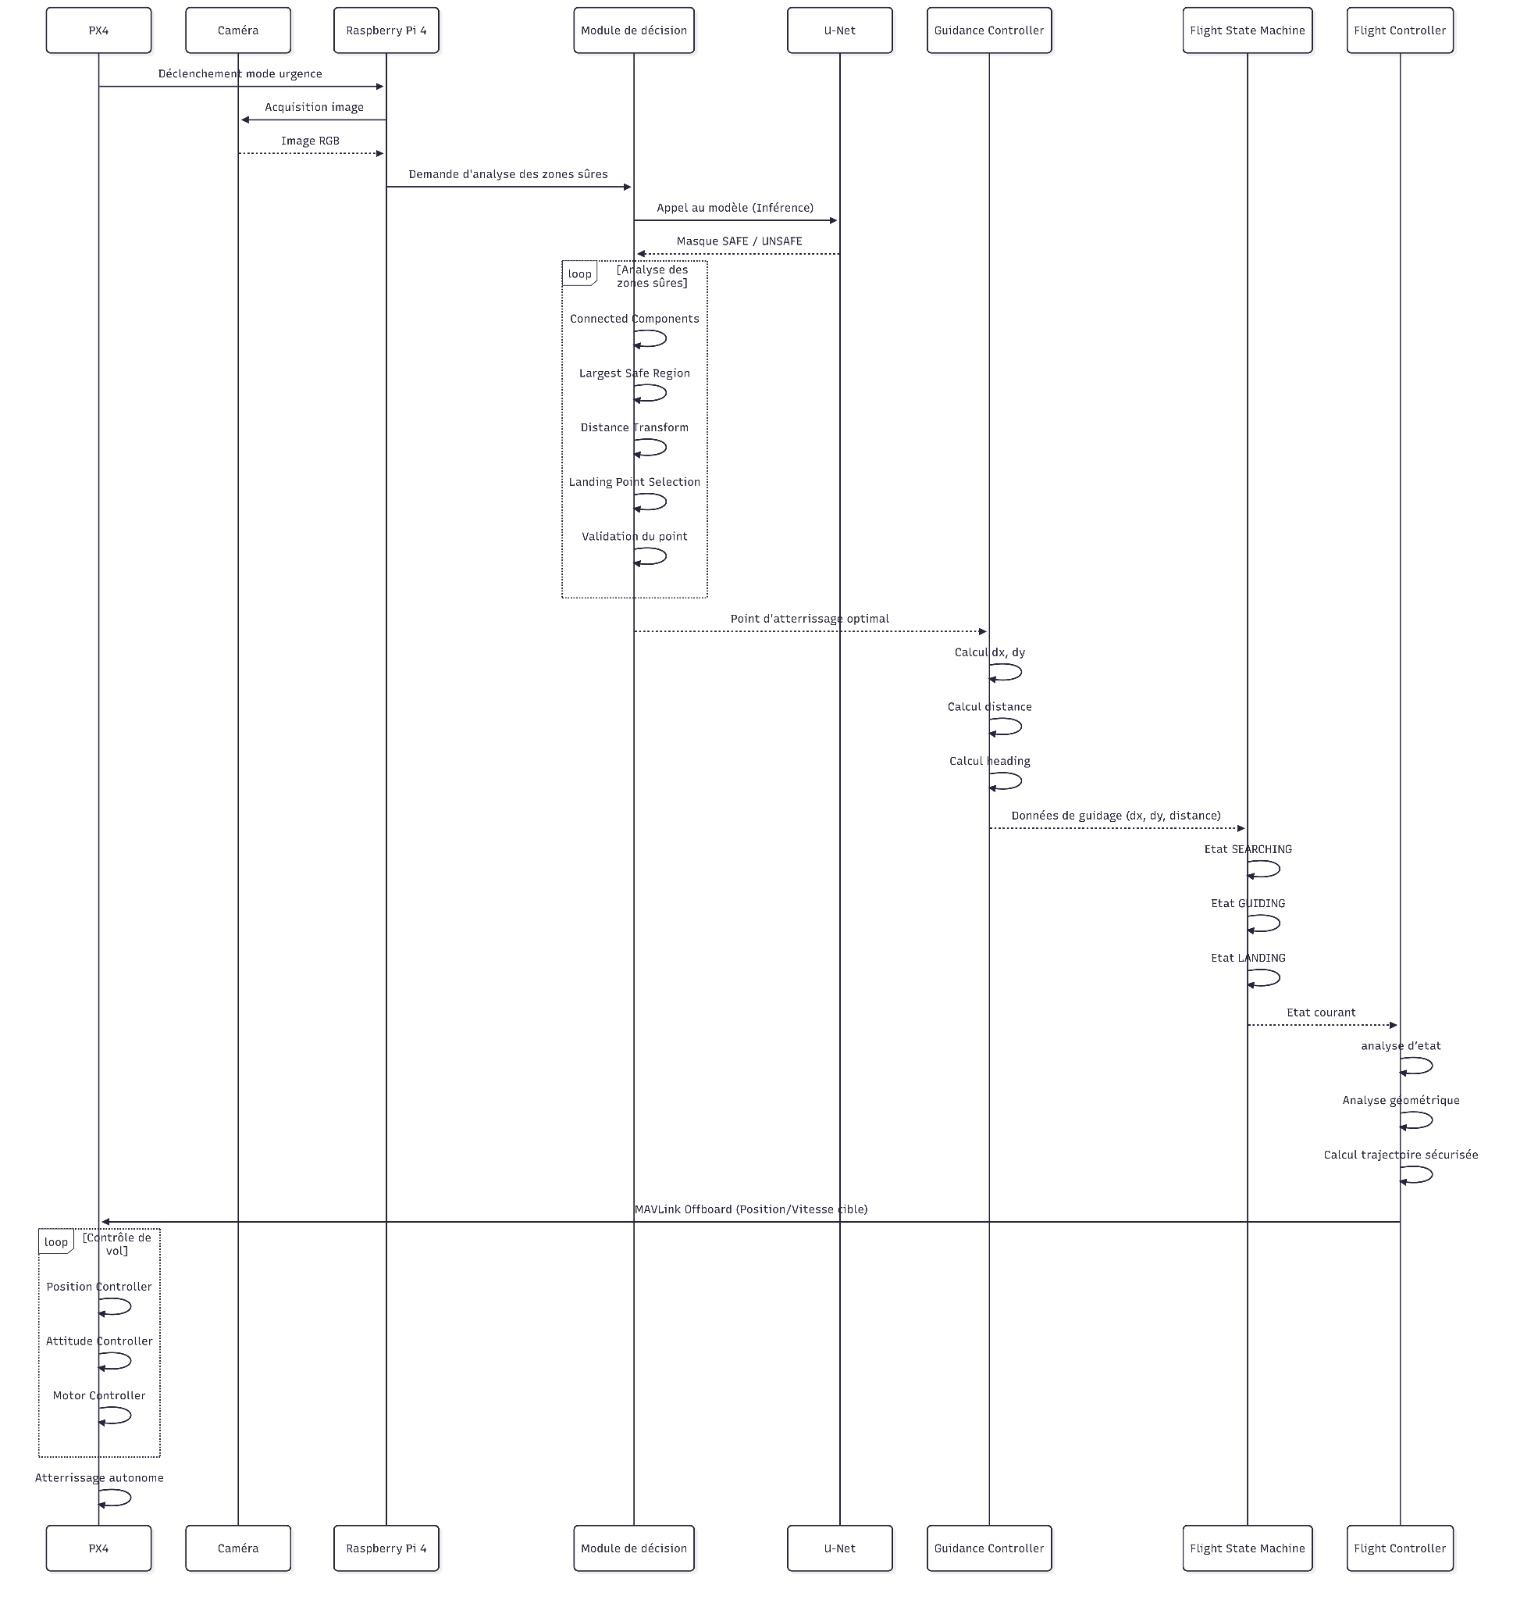
\includegraphics[width=0.7\textwidth,keepaspectratio]{assets/diagrams/sequ.jpeg}
  \caption{Flux temporel des messages entre les composants du système, incluant l'analyse des zones sûres, le calcul de guidage, la machine d'états de vol et le contrôle de vol via MAVLink.}
  \label{fig:sequence-diag}
\end{figure}

\subsection{Diagramme de composants}
\label{sec:components-diag}

Le diagramme de composants (figure~\ref{fig:components-diag}) présente l'architecture matérielle et logicielle modulaire du système global de descente d'urgence (\textit{Drone Autonomous Emergency Landing System}). L'ordinateur compagnon Raspberry Pi 4 héberge le module de vision (\textit{Vision Module}) assurant la capture caméra RGB et l'inférence par segmentation Attention U-Net. Il exécute également le module de décision (\textit{Emergency Landing System}) regroupant l'analyse des aires sûres, la sélection du point cible, le Guidance Controller, la Flight State Machine, le Flight Controller et la couche de communication avec le protocole MAVLink. En parallèle, l'autopilote PX4 intègre le module de surveillance (\textit{Monitoring Module}) alimenté par les capteurs embarqués (GPS, IMU, Baromètre), ainsi que les contrôleurs d'exécution bas niveau (Position Controller, Attitude Controller et Motor Controller) agissant sur la motorisation physique. Pour matérialiser cette conception modulaire, des choix d'outils et de technologies précis ont été retenus ; nous les détaillons dans la section suivante.

\begin{figure}[!hb]
  \centering
  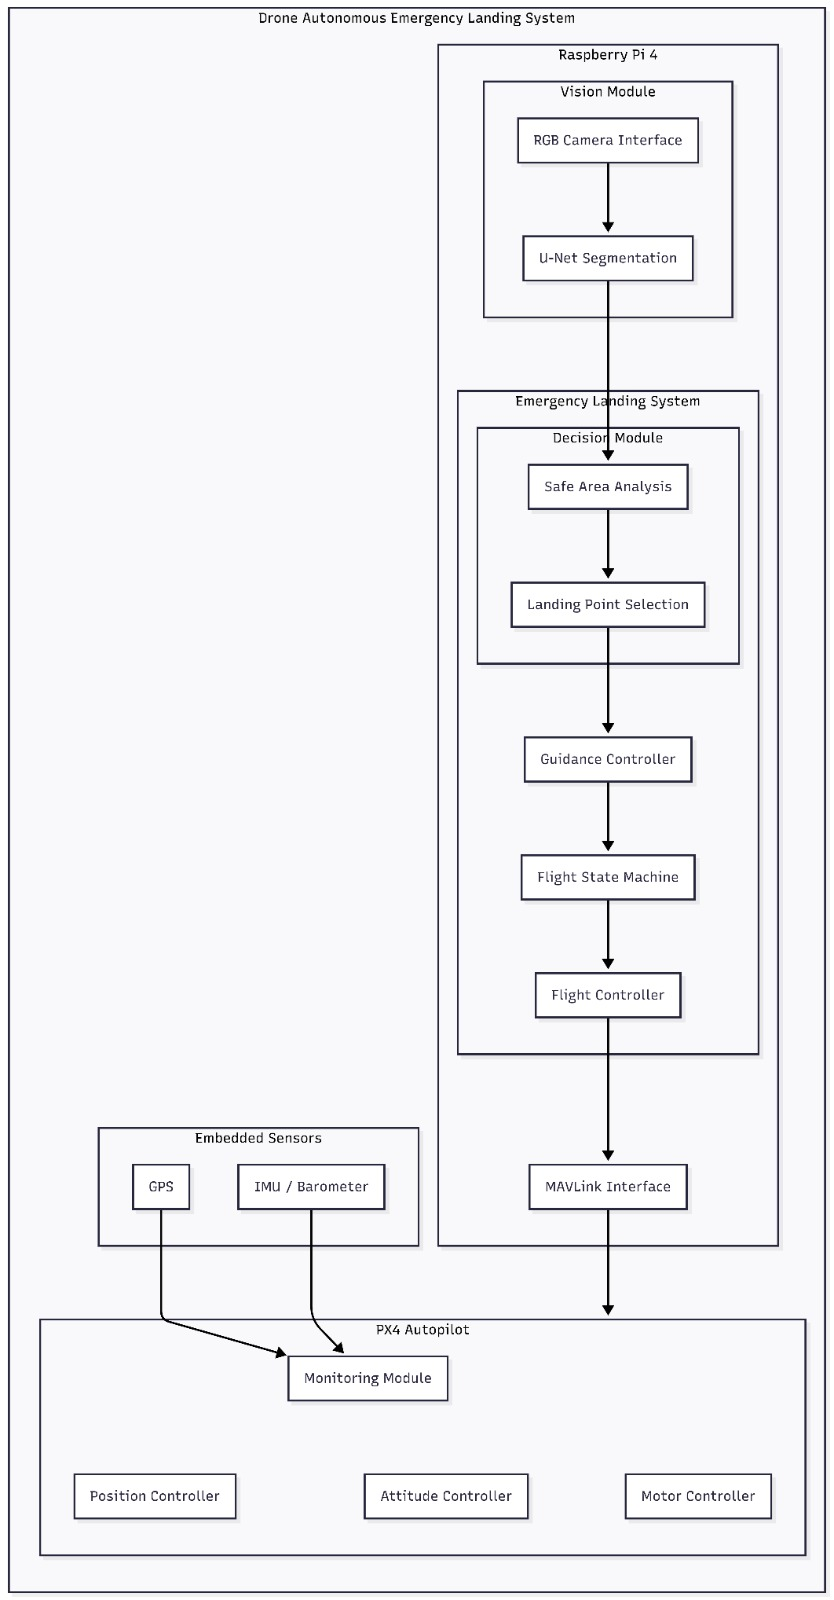
\includegraphics[width=0.55\textwidth,keepaspectratio]{assets/diagrams/compo.jpeg}
  \caption{Architecture logicielle et matérielle du système : modules de vision, de décision, de guidage et de contrôle de vol interfacés avec l'autopilote PX4 via MAVLink.}
  \label{fig:components-diag}
\end{figure}

\section{Outils et choix technologiques}
\label{sec:choix-tech}

La sélection des outils a été guidée par des critères de compatibilité, de performance, de support communautaire et de facilité de déploiement embarqué :

\vspace{0.8em}

\begin{tcolorbox}[colback=ENIADBlue!3, colframe=ENIADBlue!15, arc=4pt, boxrule=0.5pt, left=10pt, right=10pt, top=8pt, bottom=8pt]
  \begin{minipage}[c]{0.12\textwidth}
    \centering
    
\includegraphics[width=1.3cm,keepaspectratio]{images/logos/python.png}
  \end{minipage}
  \hfill
  \begin{minipage}[c]{0.84\textwidth}
    \textbf{\large Python} \\
    \textbf{Définition} : Langage de programmation dynamique de haut niveau, réputé pour sa flexibilité et la richesse de son écosystème scientifique. \\
    \textbf{Alternative} : C++ \\
    \textbf{Justification} : Retenu pour la rapidité de prototypage qu'il procure, la richesse de son écosystème de Data Science et la simplicité d'écriture des pipelines d'entraînement, bien que les modules critiques puissent être compilés par la suite pour le déploiement.
  \end{minipage}
\end{tcolorbox}

\begin{tcolorbox}[colback=ENIADBlue!3, colframe=ENIADBlue!15, arc=4pt, boxrule=0.5pt, left=10pt, right=10pt, top=8pt, bottom=8pt]
  \begin{minipage}[c]{0.12\textwidth}
    \centering
    
\includegraphics[width=1.3cm,keepaspectratio]{images/logos/pytorch.png}
  \end{minipage}
  \hfill
  \begin{minipage}[c]{0.84\textwidth}
    \textbf{\large PyTorch} \\
    \textbf{Définition} : Framework d'apprentissage profond open-source développé par Meta AI, facilitant la création et l'entraînement de réseaux de neurones. \\
    \textbf{Alternative} : TensorFlow \\
    \textbf{Justification} : Préféré pour sa conception intuitive basée sur des graphes de calcul dynamiques, simplifiant grandement le débogage et l'expérimentation rapide de l'architecture.
  \end{minipage}
\end{tcolorbox}

\begin{tcolorbox}[colback=ENIADBlue!3, colframe=ENIADBlue!15, arc=4pt, boxrule=0.5pt, left=10pt, right=10pt, top=8pt, bottom=8pt]
  \begin{minipage}[c]{0.12\textwidth}
    \centering
    
\includegraphics[width=1.3cm,keepaspectratio]{images/logos/opencv.png}
  \end{minipage}
  \hfill
  \begin{minipage}[c]{0.84\textwidth}
    \textbf{\large OpenCV} \\
    \textbf{Définition} : Bibliothèque open-source de vision par ordinateur optimisée pour le traitement d'images et la vidéo en temps réel. \\
    \textbf{Alternative} : PIL (Pillow) \\
    \textbf{Justification} : S'impose grâce à ses algorithmes natifs optimisés en C++, sa gestion des formats de caméras industrielles et sa compatibilité directe avec les tenseurs de PyTorch.
  \end{minipage}
\end{tcolorbox}

\begin{tcolorbox}[colback=ENIADBlue!3, colframe=ENIADBlue!15, arc=4pt, boxrule=0.5pt, left=10pt, right=10pt, top=8pt, bottom=8pt]
  \begin{minipage}[c]{0.12\textwidth}
    \centering
    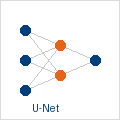
\includegraphics[width=1.3cm,keepaspectratio]{images/logos/unet.png}
  \end{minipage}
  \hfill
  \begin{minipage}[c]{0.84\textwidth}
    \textbf{\large U-Net} \\
    \textbf{Définition} : Architecture de réseau neuronal convolutif symétrique doté de skip connections, dédié à la segmentation d'images. \\
    \textbf{Alternative} : DeepLab \\
    \textbf{Justification} : Privilégié pour sa légèreté inhérente adaptée à l'Edge AI et sa capacité à préserver les frontières fines de segmentation avec un jeu de données réduit.
  \end{minipage}
\end{tcolorbox}

\begin{tcolorbox}[colback=ENIADBlue!3, colframe=ENIADBlue!15, arc=4pt, boxrule=0.5pt, left=10pt, right=10pt, top=8pt, bottom=8pt]
  \begin{minipage}[c]{0.12\textwidth}
    \centering
    
\includegraphics[width=1.3cm,keepaspectratio]{images/logos/onnx.png}
  \end{minipage}
  \hfill
  \begin{minipage}[c]{0.84\textwidth}
    \textbf{\large ONNX} \\
    \textbf{Définition} : Format ouvert et standard d'échange de modèles de Deep Learning favorisant l'interopérabilité entre outils et frameworks. \\
    \textbf{Alternative} : TorchScript \\
    \textbf{Justification} : Retenu comme format d'échange universel, permettant d'exporter et de déployer le modèle sur des cibles matérielles hétérogènes sans dépendre de l'environnement PyTorch complet.
  \end{minipage}
\end{tcolorbox}

\begin{tcolorbox}[colback=ENIADBlue!3, colframe=ENIADBlue!15, arc=4pt, boxrule=0.5pt, left=10pt, right=10pt, top=8pt, bottom=8pt]
  \begin{minipage}[c]{0.12\textwidth}
    \centering
    
\includegraphics[width=1.3cm,keepaspectratio]{images/logos/tensorrt.png}
  \end{minipage}
  \hfill
  \begin{minipage}[c]{0.84\textwidth}
    \textbf{\large TensorRT} \\
    \textbf{Définition} : Kit de développement logiciel de NVIDIA optimisant les modèles pour l'inférence hautes performances sur processeur graphique. \\
    \textbf{Alternative} : OpenVINO \\
    \textbf{Justification} : Choisi car notre cible matérielle finale repose sur l'architecture NVIDIA (ex. Jetson Orin), garantissant des accélérations d'inférence maximales grâce à une compilation matérielle spécifique.
  \end{minipage}
\end{tcolorbox}

\begin{tcolorbox}[colback=ENIADBlue!3, colframe=ENIADBlue!15, arc=4pt, boxrule=0.5pt, left=10pt, right=10pt, top=8pt, bottom=8pt]
  \begin{minipage}[c]{0.12\textwidth}
    \centering
    
\includegraphics[width=1.3cm,keepaspectratio]{images/logos/cuda.png}
  \end{minipage}
  \hfill
  \begin{minipage}[c]{0.84\textwidth}
    \textbf{\large CUDA} \\
    \textbf{Définition} : Architecture de calcul parallèle et API développée par NVIDIA pour accélérer les traitements intensifs sur GPU. \\
    \textbf{Alternative} : CPU \\
    \textbf{Justification} : Indispensable pour la parallélisation massive des calculs matriciels du réseau, permettant d'inférer 10 fois plus vite et de satisfaire les impératifs du temps réel requis pour le guidage.
  \end{minipage}
\end{tcolorbox}

\subsection{Écosystème matériel et protocoles pour l'intégration drone}
\label{subsec:ecosysteme-drone}

Bien que l'implémentation actuelle de ce projet ait été réalisée et validée de manière logicielle et hors ligne (sans tests physiques sur machine volante), l'intégration réelle du système sur un vecteur aérien autonome implique un écosystème spécifique d'outils matériels et de protocoles de communication. Les fiches suivantes détaillent ces composants clés pour un futur déploiement embarqué :

\vspace{0.8em}

\begin{tcolorbox}[colback=ENIADBlue!3, colframe=ENIADBlue!15, arc=4pt, boxrule=0.5pt, left=10pt, right=10pt, top=8pt, bottom=8pt]
  \begin{minipage}[c]{0.12\textwidth}
    \centering
    
\includegraphics[width=1.3cm,keepaspectratio]{images/logos/mavlink.png}
  \end{minipage}
  \hfill
  \begin{minipage}[c]{0.84\textwidth}
    \textbf{\large MAVLink} \\
    \textbf{Définition} : Protocole de communication binaire léger sous forme de sérialisation de messages, conçu pour l'échange d'informations entre un pilote automatique et des composants embarqués ou stations sol. \\
    \textbf{Utilité potentielle} : Permettrait de transmettre en temps réel les coordonnées du point d'atterrissage optimal calculées par le module de vision vers l'autopilote et de récupérer la télémétrie du drone (altitude, attitude). \\
    \textbf{Statut d'utilisation} : \textbf{Non intégré / Non utilisé} dans l'implémentation physique actuelle de ce projet, constituant une perspective d'intégration matérielle.
  \end{minipage}
\end{tcolorbox}

\begin{tcolorbox}[colback=ENIADBlue!3, colframe=ENIADBlue!15, arc=4pt, boxrule=0.5pt, left=10pt, right=10pt, top=8pt, bottom=8pt]
  \begin{minipage}[c]{0.12\textwidth}
    \centering
    
\includegraphics[width=1.3cm,keepaspectratio]{images/logos/raspberrypi.png}
  \end{minipage}
  \hfill
  \begin{minipage}[c]{0.84\textwidth}
    \textbf{\large Raspberry Pi} \\
    \textbf{Définition} : Ordinateur monocarte à basse consommation d'énergie fonctionnant sous Linux, fréquemment configuré comme calculateur compagnon à bord du drone. \\
    \textbf{Utilité potentielle} : Servirait d'unité d'acquisition d'images de la caméra et de traitement d'inférence sémantique légère avant de piloter le contrôleur de vol principal via liaison série. \\
    \textbf{Statut d'utilisation} : \textbf{Non intégré / Non utilisé} dans l'implémentation physique actuelle de ce projet, les calculs ayant été validés hors ligne sur GPU de développement.
  \end{minipage}
\end{tcolorbox}

\begin{tcolorbox}[colback=ENIADBlue!3, colframe=ENIADBlue!15, arc=4pt, boxrule=0.5pt, left=10pt, right=10pt, top=8pt, bottom=8pt]
  \begin{minipage}[c]{0.12\textwidth}
    \centering
    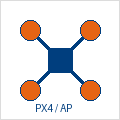
\includegraphics[width=1.3cm,keepaspectratio]{images/logos/px4.png}
  \end{minipage}
  \hfill
  \begin{minipage}[c]{0.84\textwidth}
    \textbf{\large PX4 / ArduPilot} \\
    \textbf{Définition} : Logiciels de contrôle de vol (\textit{firmwares}) de référence pour pilotes automatiques, assurant la stabilisation physique, le suivi de trajectoire et l'évitement d'obstacles bas niveau. \\
    \textbf{Utilité potentielle} : Géreraient la dynamique physique de vol et exécuteraient la commande de descente ou d'évitement reçue du compagnon de calcul IA via des ordres standardisés. \\
    \textbf{Statut d'utilisation} : \textbf{Non intégré / Non utilisé} dans l'implémentation physique actuelle de ce projet, le guidage ayant été modélisé de façon logicielle dans le notebook.
  \end{minipage}
\end{tcolorbox}

\vspace{0.8em}

Ces choix et perspectives offrent un compromis équilibré entre performance, précision et simplicité de déploiement, posant les bases techniques détaillées dans les chapitres suivants.

\vspace{1.5em}
\textbf{Conclusion}

En conclusion, ce deuxième chapitre a permis de traduire la problématique globale du projet en exigences fonctionnelles et non fonctionnelles concrètes. La modélisation de l'architecture par les diagrammes de séquence et de composants, conjuguée à la justification minutieuse de nos choix technologiques (Python, PyTorch, OpenCV, ONNX), a permis de définir une solution modulaire et optimale pour un environnement embarqué GPU. Fort de cette conception logicielle et matérielle validée, le chapitre suivant se penchera sur la mise en œuvre pratique en décrivant la préparation des données, le pipeline d'augmentation, et les étapes clés du développement de notre modèle de segmentation profonde.


\clearpage

% ============================================================
%  CHAPITRE 3 — DONNÉES ET DÉVELOPPEMENT DU MODÈLE
% ============================================================
\chapter{Données et Développement du Modèle}
\label{chap:dataset}
\label{chap:modele}

\section{Introduction}

La qualité du dataset, la robustesse du prétraitement et la conception de l'architecture du réseau de neurones conditionnent directement les performances du système de segmentation. Avant qu'un modèle puisse distinguer une surface praticable d'un obstacle dangereux, les données doivent être validées, harmonisées, enrichies et optimisées pour le chargement. Ce chapitre présente le dataset utilisé, son exploration statistique, la chaîne de prétraitement appliquée, ainsi que le développement de l'architecture profonde (Attention U-Net) et du mécanisme de décision géométrique permettant de sélectionner automatiquement la meilleure zone d'atterrissage. Nous commençons par étudier la source de nos données en présentant les spécificités du jeu de données aériennes retenu.

\section{Présentation et exploration du dataset}
\label{sec:dataset-exploration}

Le projet s'appuie sur le \textbf{Graz Semantic Drone Dataset}~\cite{graz2015semantic}, une base publique de segmentation sémantique constituée d'images aériennes (\textit{vue top-down}) capturées entre 5 et 30 mètres d'altitude, couvrant des zones urbaines, périurbaines, des espaces naturels et des surfaces mixtes — des conditions représentatives d'un atterrissage d'urgence réel.

\begin{table}[!hb]
  \centering
  \caption{Caractéristiques du Graz Semantic Drone Dataset.}
  \label{tab:dataset-stats}
  \renewcommand{\arraystretch}{1.4}
  \begin{tabularx}{0.7\textwidth}{
    >{\bfseries\color{ENIADBlue}}l
    >{\centering\arraybackslash}X
  }
    \toprule
    \rowcolor{ENIADBlue!12}
    \textbf{Élément} & \textbf{Valeur} \\
    \midrule
    Nombre d'images / masques & 400 \\
    \rowcolor{ENIADLightBlue!20}
    Résolution originale & jusqu'à $6000 \times 4000$ px \\
    Résolution standardisée & $320 \times 320$ px \\
    \rowcolor{ENIADLightBlue!20}
    Classes sémantiques & 24 \\
    \bottomrule
  \end{tabularx}
\end{table}

Les 24 classes sémantiques sont regroupées en quatre catégories fonctionnelles :

\begin{table}[!hb]
  \centering
  \caption{Regroupement fonctionnel des 24 classes sémantiques.}
  \label{tab:classes}
  \renewcommand{\arraystretch}{1.4}
  \begin{tabularx}{0.95\textwidth}{
    >{\bfseries\color{ENIADBlue}}l
    >{\arraybackslash}X
  }
    \toprule
    \rowcolor{ENIADBlue!12}
    \textbf{Catégorie} & \textbf{Classes} \\
    \midrule
    Surfaces d'atterrissage potentielles & paved-area, grass, dirt, gravel \\
    \rowcolor{ENIADLightBlue!20}
    Obstacles critiques & person, dog, car, bicycle, water, pool \\
    Structures verticales & tree, bald-tree, vegetation, roof, wall, window, door, fence, fence-pole \\
    \rowcolor{ENIADLightBlue!20}
    Classes diverses & rocks, ar-marker, obstacle, conflicting, unlabeled \\
    \bottomrule
  \end{tabularx}
\end{table}

Pour le calcul du score de sécurité (décrit plus loin dans ce chapitre), ces classes sont regroupées en deux ensembles binaires : \textbf{Safe Classes} (paved-area, grass) et \textbf{Critical Obstacles} (person, dog, car, water).

\textbf{\textcolor{red}{Note :}} L'analyse exploratoire (EDA) révèle un déséquilibre marqué entre classes dominantes (\textit{paved-area}, \textit{grass}, \textit{roof}, \textit{tree}) et classes minoritaires (\textit{person}, \textit{dog}, \textit{bicycle}). Ce déséquilibre a directement motivé le choix de la Tversky Loss combinée à la Binary Cross Entropy, détaillé dans la suite de ce chapitre.

Pour exploiter ces classes de manière robuste malgré leur déséquilibre, les données brutes doivent subir une série de transformations et de normalisations que nous détaillons ci-après.

\section{Annotation et prétraitement}
\label{sec:pretraitement}

Chaque masque est stocké au format RGB, chaque couleur correspondant à une classe (ex. \texttt{[255,22,96]} $\rightarrow$ \textit{person}, \texttt{[0,102,0]} $\rightarrow$ \textit{grass}, \texttt{[128,64,128]} $\rightarrow$ \textit{paved-area}). Le pipeline de prétraitement, implémenté dans \texttt{DroneDataset} (\texttt{dataset.py}), applique successivement :

\begin{enumerate}[leftmargin=2em, itemsep=4pt, label=\textbf{\arabic*.}]
  \item \textbf{Validation} des paires image/masque (présence, correspondance des noms) via \texttt{\_validate\_coherence()} ;
  \item \textbf{Redimensionnement} à $320 \times 320$, avec interpolation linéaire pour les images et plus proche voisin pour les masques (afin de préserver les frontières de classes) ;
  \item \textbf{Normalisation} selon les statistiques ImageNet (moyenne $(0.485, 0.456, 0.406)$, écart-type $(0.229, 0.224, 0.225)$), nécessaire à la compatibilité avec l'encodeur EfficientNet-B0 pré-entraîné et à l'accélération de la convergence ;
  \item \textbf{Encodage LUT} des masques : chaque couleur RGB est convertie en un indice de classe via un hash \texttt{(R<<16)+(G<<8)+B}, réduisant fortement le temps de chargement CPU.
\end{enumerate}

\subsection{Augmentation des données (Data Augmentation)}
\label{subsec:data-augmentation}

Pour pallier la taille limitée de notre dataset (400 images) et prévenir tout risque de surapprentissage, un pipeline d'augmentation robuste basé sur la bibliothèque \texttt{Albumentations}~\cite{buslaev2020albumentations} a été conçu. Les transformations appliquées visent à simuler la diversité des scènes de vol réelles à travers quatre catégories fonctionnelles :

\begin{itemize}[leftmargin=1.8em, itemsep=4pt]
  \item \textbf{Robustesse géométrique} :
    \begin{itemize}[label=\textbullet, leftmargin=1.2em]
      \item \texttt{HorizontalFlip} ($p = 0.5$) et \texttt{VerticalFlip} ($p = 0.3$) : symétries axiales simulant des changements d'orientation de vol.
      \item \texttt{RandomRotate90} ($p = 0.5$) : rotation libre à $90^\circ$, idéale pour les prises de vue aériennes zénithales (\textit{top-down}) où l'orientation absolue n'a pas d'influence sémantique.
      \item \texttt{ShiftScaleRotate} ($p = 0.7$) : translation (limite $0.1$), échelle (limite $0.2$) et rotation (limite $30^\circ$) avec un mode de bordure par réflexion (\texttt{BORDER\_REFLECT\_101}) pour éviter les zones noires artificielles.
      \item \texttt{Perspective} ($p = 0.3$, échelle $0.04$ à $0.08$) : déformation de perspective simulant les inclinaisons angulaires de la caméra embarquée lors des mouvements de tangage et de roulis du drone.
    \end{itemize}
  \item \textbf{Robustesse photométrique} :
    \begin{itemize}[label=\textbullet, leftmargin=1.2em]
      \item \texttt{RandomBrightnessContrast} ($p = 0.6$, limite $0.3$) : ajustement aléatoire de la luminosité et du contraste pour faire face aux variations d'ensoleillement et d'exposition.
    \end{itemize}
  \item \textbf{Simulation de conditions météo et environnementales} :
    \begin{itemize}[label=\textbullet, leftmargin=1.2em]
      \item \texttt{RandomShadow} ($p = 0.3$) et \texttt{RandomFog} ($p = 0.2$) : ajout d'ombres portées et de brouillard artificiels, indispensables pour garantir la détection d'obstacles dans des environnements ombragés ou par temps couvert.
    \end{itemize}
  \item \textbf{Régularisation et normalisation} :
    \begin{itemize}[label=\textbullet, leftmargin=1.2em]
      \item \texttt{CoarseDropout} ($p = 0.3$, max. 8 trous de $32\times32$ px) : suppression aléatoire de rectangles de l'image (Cutout) pour forcer le modèle à apprendre des caractéristiques contextuelles globales et à tolérer les occlusions partielles d'obstacles.
      \item \texttt{Normalize} ($p = 1.0$) : normalisation finale centrée-réduite basée sur les statistiques ImageNet (moyenne $[0.485, 0.456, 0.406]$ et écart-type $[0.229, 0.224, 0.225]$) pour aligner les données avec les poids pré-entraînés du réseau.
    \end{itemize}
\end{itemize}

L'extrait de code suivant, tiré de notre script d'entraînement (annexe~\ref{sec:code-dataset-augmentation}), illustre la mise en œuvre de cette chaîne d'augmentation :

\begin{lstlisting}[language=Python, caption={Définition du pipeline d'augmentation des données via Albumentations.}]
train_transform = A.Compose([
    A.Resize(320, 320),
    A.HorizontalFlip(p=0.5),
    A.VerticalFlip(p=0.3),
    A.RandomRotate90(p=0.5),
    A.ShiftScaleRotate(
        shift_limit=0.1, scale_limit=0.2, rotate_limit=30,
        border_mode=cv2.BORDER_REFLECT_101, p=0.7
    ),
    A.Perspective(scale=(0.04, 0.08), p=0.3),
    A.RandomBrightnessContrast(brightness_limit=0.3, contrast_limit=0.3, p=0.6),
    A.CoarseDropout(
        max_holes=8, max_height=32, max_width=32,
        min_holes=1, fill_value=0, mask_fill_value=0, p=0.3
    ),
    A.Normalize(mean=(0.485, 0.456, 0.406), std=(0.229, 0.224, 0.225)),
    ToTensorV2(),
])
\end{lstlisting}

Après avoir préparé et enrichi ces images par cette chaîne d'augmentations, il convient de répartir équitablement le jeu de données pour l'entraînement et l'évaluation, ce qui fait l'objet de la section suivante.

\section{Séparation des données}
\label{sec:separation}

Le dataset a été réparti selon un ratio classique :

\begin{table}[!ht]
  \centering
  \caption{Répartition du dataset en ensembles d'entraînement, validation et test.}
  \label{tab:split}
  \renewcommand{\arraystretch}{1.4}
  \begin{tabularx}{0.65\textwidth}{
    >{\bfseries\color{ENIADBlue}}l
    >{\centering\arraybackslash}X
    >{\centering\arraybackslash}X
  }
    \toprule
    \rowcolor{ENIADBlue!12}
    \textbf{Ensemble} & \textbf{Ratio} & \textbf{Images} \\
    \midrule
    Entraînement & 70~\% & 280 \\
    \rowcolor{ENIADLightBlue!20}
    Validation & 15~\% & 60 \\
    Test & 15~\% & 60 \\
    \bottomrule
  \end{tabularx}
\end{table}

Une fois le dataset ainsi préparé, nettoyé et divisé en sous-ensembles d'apprentissage, de validation et de test, il peut alimenter la chaîne de traitement intelligente. La section suivante détaille le pipeline complet d'intelligence artificielle qui exploite ces données pour aboutir à la décision finale d'atterrissage sécurisé.

\section{Pipeline IA complet}
\label{sec:pipeline}

Le système transforme une scène aérienne brute en une décision d'atterrissage exploitable à travers une chaîne séquentielle organisée en quatre grandes phases thématiques (figure~\ref{fig:pipeline-global}) : la phase d'acquisition (bleue, englobant la capture vidéo de la caméra et le prétraitement d'image), la phase de segmentation et décision (orange, comprenant l'inférence du modèle U-Net pour la génération du masque sémantique binaire et la sélection de zone par l'analyse des zones sûres), la phase de guidage et contrôle (verte, associant la machine d'états pour la gestion des états, le Guidance Controller et le Flight Controller assurant les commandes bas niveau), et enfin la phase de communication et d'actionnement (grise, regroupant le protocole MAVLink pour la communication standard, le firmware de vol PX4/ArduPilot et l'exécution physique sur le drone).

\begin{figure}[!ht]
  \centering
  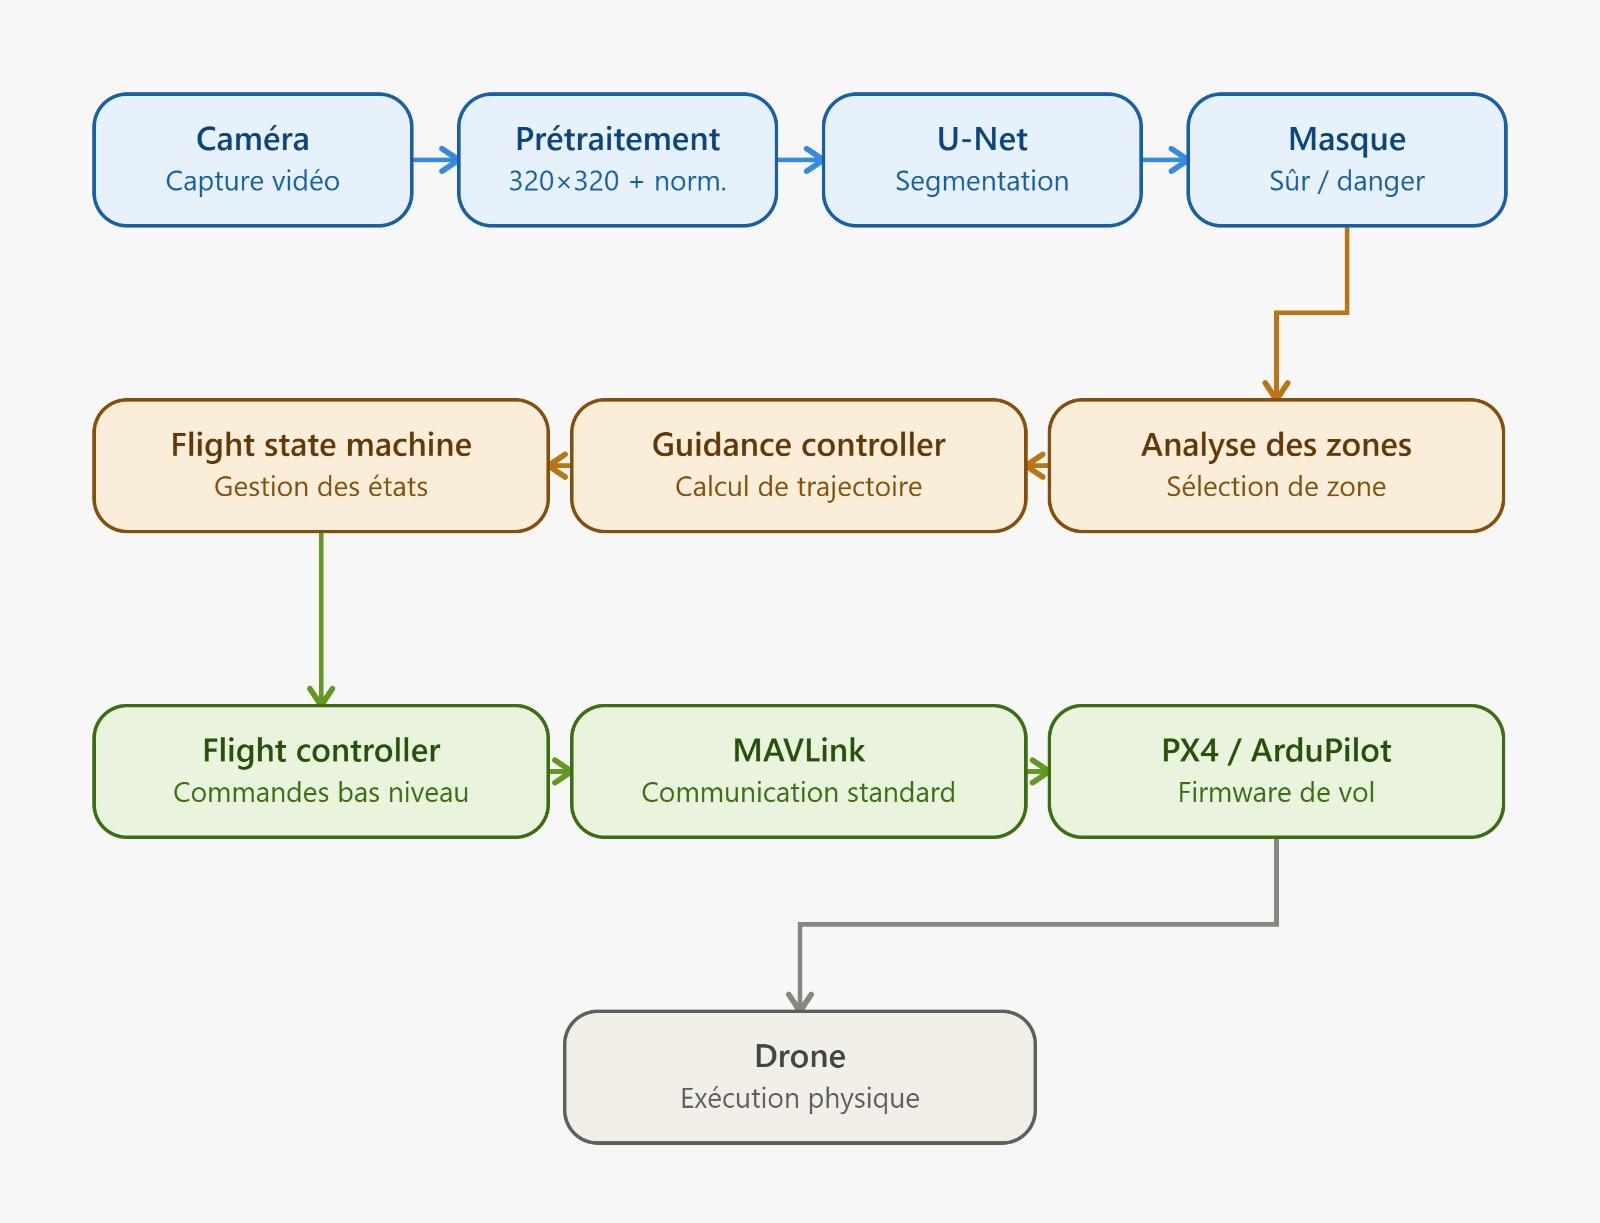
\includegraphics[width=0.8\textwidth,keepaspectratio]{1.jpeg}
  \caption{Pipeline global du système d'atterrissage autonome, depuis la capture caméra jusqu'à l'exécution physique sur le drone via PX4/ArduPilot.}
  \label{fig:pipeline-global}
\end{figure}

À partir du masque sémantique binaire, le système calcule une Distance Transform entre chaque région praticable et les obstacles détectés, puis évalue un score de sécurité pour identifier automatiquement la zone offrant le meilleur niveau de sûreté. Les étapes de ce traitement, depuis la prédiction du masque jusqu'à l'extraction de la zone la plus sûre, sont illustrées dans la figure~\ref{fig:best-landing-point}.

\begin{figure}[!hb]
  \centering
  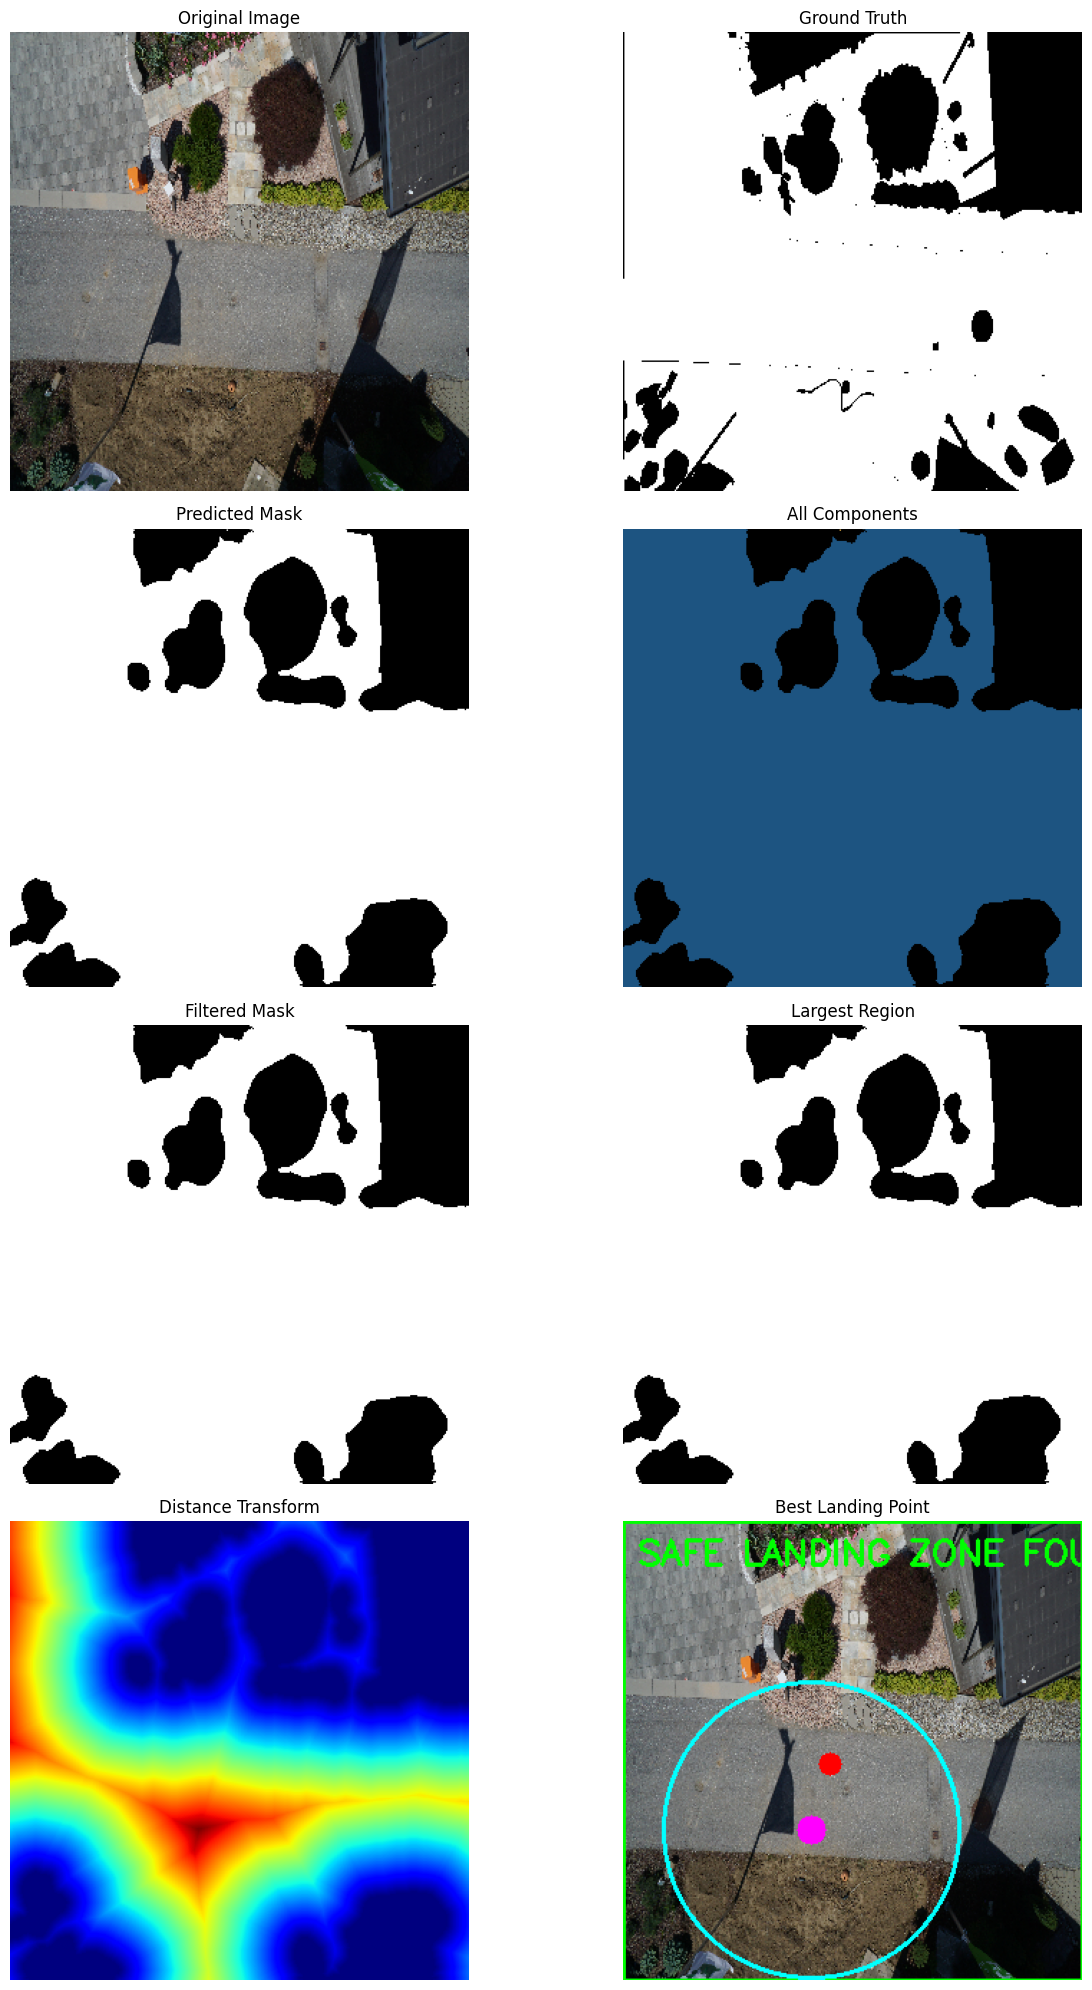
\includegraphics[width=0.5\textwidth,keepaspectratio]{assets/model/best_landing_point.png}
  \caption{Étapes de détection de la zone d'atterrissage la plus sûre (\textit{best area}) : image originale, vérité terrain, masque prédit, composantes connexes, masque filtré par aire minimale ($5000$ px), sélection de la plus grande région, application de la Distance Transform et localisation du point d'atterrissage optimal.}
  \label{fig:best-landing-point}
\end{figure}

Ce pipeline décisionnel repose au premier plan sur les algorithmes de guidage et de pilotage décrits dans la section suivante.

\section{Contrôleur de guidage et machine d'états}
\label{sec:guidage-state-machine}

Une fois la zone d'atterrissage optimale identifiée par le pipeline de vision, les coordonnées du point cible doivent être converties en commandes de vol pour guider le drone de manière autonome. Cette logique de pilotage de haut niveau associe un contrôleur de guidage géométrique et une machine d'états de vol.

\subsection{Sélection du point d'atterrissage optimal}

Le module d'analyse extrait les composantes connexes du masque de pixels sûrs. Les zones dont l'aire est inférieure à un seuil critique de sécurité ($5000$ pixels dans notre implémentation) sont exclues afin d'éviter tout atterrissage dans des clairières exiguës ou à proximité immédiate d'obstacles. Sur la plus grande composante connexe retenue, la Distance Transform euclidienne est calculée. L'algorithme recherche ensuite le point maximisant cette distance via \texttt{cv2.minMaxLoc()}, ce qui correspond au centre du plus grand cercle exempt d'obstacles inscrit dans la zone. Ce point, qui garantit la plus grande marge de sécurité physique par rapport aux menaces environnantes, est alors transmis au module de guidage.

\subsection{Contrôleur de guidage géométrique}

Le contrôleur de guidage, dont l'implémentation est détaillée à l'annexe~\ref{sec:code-guidage-machine}, calcule à chaque cycle l'erreur horizontale ($dx$) et verticale ($dy$) entre le centre de l'image (représentant la position actuelle du drone en vol stationnaire zénithal) et les coordonnées du point cible :
\begin{equation}
  dx = X_{\text{cible}} - X_{\text{centre}}, \quad dy = Y_{\text{cible}} - Y_{\text{centre}}
\end{equation}
La distance euclidienne $D = \sqrt{dx^2 + dy^2}$ et l'angle de gisement (\textit{heading}) $\theta = \arctan2(dy, dx)$ sont calculés pour orienter le drone. Une zone de tolérance de $\pm 10$ pixels est appliquée : si l'écart dépasse ce seuil, le contrôleur émet des commandes directionnelles discrètes (\texttt{MOVE LEFT}, \texttt{MOVE RIGHT}, \texttt{MOVE FORWARD}, \texttt{MOVE BACKWARD}), sinon il passe en commande stationnaire (\texttt{HOLD}) et active le signal de centrage.

\subsection{Machine d'états de vol}

Pour orchestrer le comportement dynamique du drone en situation d'urgence, une machine d'états à trois modes est définie (figure~\ref{fig:guidance-visualisation}) :
\begin{itemize}[leftmargin=1.8em, itemsep=4pt]
  \item \textbf{SEARCHING} : Le drone balaie la zone à la recherche d'une surface praticable d'une aire minimale requise. Dès qu'une zone valide est détectée et autorisée par le score de sécurité, le système bascule vers l'état \textbf{GUIDING}.
  \item \textbf{GUIDING} : Le drone applique les commandes générées par le contrôleur de guidage pour se déplacer en translation vers le point d'atterrissage optimal. Si la zone devient indisponible ou obstruée, il retourne à l'état \textbf{SEARCHING} ; si le drone parvient à se centrer au-dessus de la cible dans la tolérance admise, il transite vers l'état \textbf{LANDING}.
  \item \textbf{LANDING} : Le drone déclenche sa descente verticale finale. Si un obstacle surgit durant la descente, la machine d'états interrompt la procédure et réactive l'état \textbf{SEARCHING} pour trouver une zone alternative.
\end{itemize}

\begin{figure}[!hb]
  \centering
  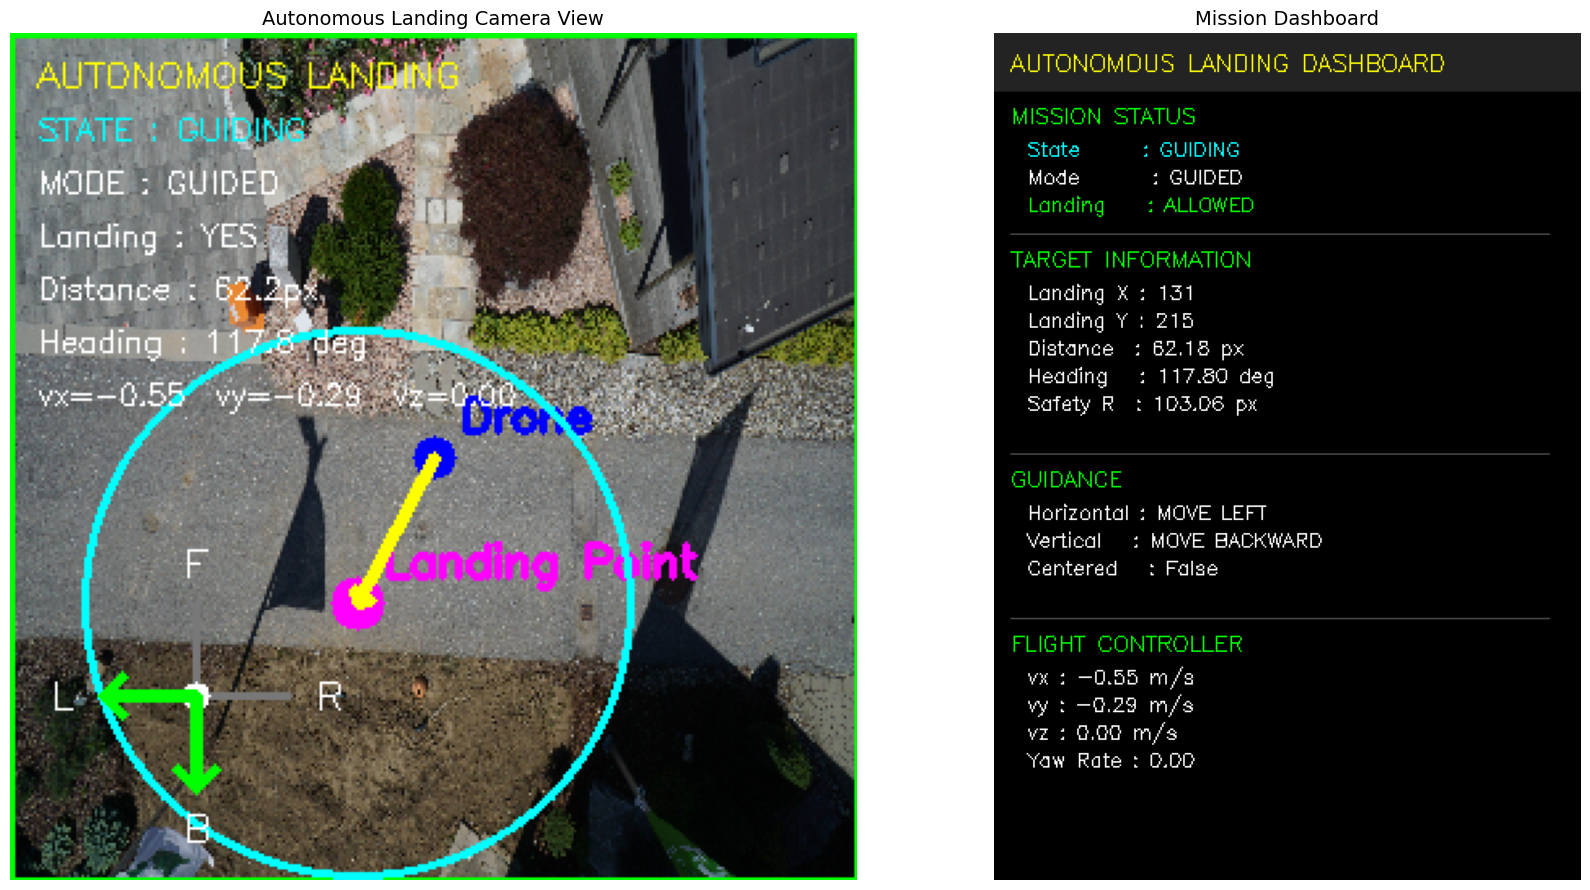
\includegraphics[width=0.55\textwidth,keepaspectratio]{assets/model/guidance_visualisation_v2.png}
  \caption{Visualisation de guidage finale (drone centré sur la zone d'atterrissage sélectionnée).}
  \label{fig:guidance-visualisation}
\end{figure}

\subsection{Contrôleur de vol (Flight Controller)}
\label{subsec:flight-controller}

Le module final de la chaîne de décision est le contrôleur de vol (\textit{Flight Controller}). Ce module sert de couche d'adaptation logique entre les commandes géométriques de haut niveau et le pilotage bas niveau du drone.

Concrètement, le contrôleur de vol reçoit à chaque itération l'état courant de la machine d'états de vol (\texttt{SEARCHING}, \texttt{GUIDING} ou \texttt{LANDING}) ainsi que les consignes directionnelles calculées par le contrôleur de guidage (\texttt{MOVE LEFT}, \texttt{MOVE RIGHT}, \texttt{MOVE FORWARD}, \texttt{MOVE BACKWARD} ou \texttt{HOLD}). Son rôle est d'interpréter ces données pour générer des consignes de vitesses tridimensionnelles ($v_x$, $v_y$, $v_z$) et de taux de lacet (\textit{yaw rate}) adaptées aux attentes de l'autopilote :
\begin{itemize}[leftmargin=1.8em, itemsep=4pt]
  \item En état \textbf{SEARCHING} : Les vitesses de translation sont maintenues nulles, et le drone effectue un balayage rotatif lent pour acquérir de nouvelles images.
  \item En état \textbf{GUIDING} : Les commandes discrètes du guidage (ex. \texttt{MOVE FORWARD}) sont converties en vitesses de translation proportionnelles (ex. $v_x = 0.5$ m/s), tout en maintenant l'altitude constante.
  \item En état \textbf{LANDING} : Les vitesses horizontales sont annulées, et une vitesse verticale de descente contrôlée ($v_z = -0.25$ m/s) est commandée jusqu'au toucher du sol.
\end{itemize}

Ces consignes sont conçues pour être encapsulées sous forme de messages du protocole \textit{MAVLink} afin d'être transmises au micrologiciel de l'autopilote (comme PX4 ou ArduPilot) via une liaison série ou réseau. Dans le cadre de ce projet, ce module de commande de vol a été implémenté et évalué de façon logicielle hors ligne (sur flux d'images statiques de test), jetant les bases algorithmiques requises pour une validation future sur drone physique. L'implémentation complète de cette interface logique et de la machine de vol est fournie à l'annexe~\ref{sec:code-guidage-machine}.

Ce pipeline de guidage et de contrôle de vol complète notre système intelligent en aval de la segmentation sémantique. L'architecture profonde qui permet d'obtenir le masque sémantique de départ est détaillée dans la section suivante.

\section{Architecture du modèle}
\label{sec:architecture-modele}

Le réseau suit le principe de l'architecture Attention U-Net~\cite{oktay2018attention} enrichi d'un encodeur EfficientNet-B0~\cite{tan2019efficientnet} pré-entraîné et de connexions résiduelles.

\subsection{Encodeur — EfficientNet-B0}

EfficientNet-B0 extrait progressivement les caractéristiques de l'image par niveaux successifs, la résolution spatiale diminuant à mesure que la richesse sémantique augmente :

\begin{table}[!ht]
  \centering
  \caption{Niveaux de l'encodeur EfficientNet-B0.}
  \label{tab:encodeur}
  \renewcommand{\arraystretch}{1.4}
  \begin{tabularx}{0.65\textwidth}{
    >{\bfseries\color{ENIADBlue}}c
    >{\centering\arraybackslash}X
    >{\centering\arraybackslash}X
  }
    \toprule
    \rowcolor{ENIADBlue!12}
    \textbf{Niveau} & \textbf{Canaux} & \textbf{Taille} \\
    \midrule
    Bloc 1 & 16 & $160\times160$ \\
    \rowcolor{ENIADLightBlue!20}
    Bloc 2 & 24 & $80\times80$ \\
    Bloc 3 & 40 & $40\times40$ \\
    \rowcolor{ENIADLightBlue!20}
    Bloc 4 & 112 & $20\times20$ \\
    Bloc 5 & 320 & $10\times10$ \\
    \bottomrule
  \end{tabularx}
\end{table}

\subsection{Skip connections}

Pour limiter la perte d'informations fines lors de la compression, des connexions résiduelles (skip connections) transfèrent directement les cartes de caractéristiques haute résolution de l'encodeur vers le décodeur, améliorant la reconstruction spatiale et la précision des contours.

\subsection{Sortie}

Une convolution finale $1\times1$ réduit les caractéristiques à 1 seule carte, convertie en probabilités par une fonction Sigmoïde afin d'obtenir un masque binaire final indiquant si la zone est praticable (SAFE) ou non (UNSAFE). La définition de cette architecture étant posée, son apprentissage nécessite de configurer des hyperparamètres précis, détaillés dans la section suivante.

\section{Hyperparamètres et configuration d'entraînement}
\label{sec:hyperparams}

\begin{table}[!ht]
  \centering
  \caption{Hyperparamètres d'entraînement du modèle.}
  \label{tab:hyperparams}
  \renewcommand{\arraystretch}{1.4}
  \begin{tabularx}{0.75\textwidth}{
    >{\bfseries\color{ENIADBlue}}l
    >{\centering\arraybackslash}X
  }
    \toprule
    \rowcolor{ENIADBlue!12}
    \textbf{Paramètre} & \textbf{Valeur} \\
    \midrule
    Époques max. & 150 (Early Stopping à 128) \\
    \rowcolor{ENIADLightBlue!20}
    Batch Size & 8 \\
    Learning Rate & 0.0003 \\
    \rowcolor{ENIADLightBlue!20}
    Optimiseur & AdamW~\cite{loshchilov2019adamw} \\
    Weight Decay & 0.0001 \\
    \rowcolor{ENIADLightBlue!20}
    Scheduler & Cosine Annealing (avec redémarrages)~\cite{loshchilov2017sgdr} \\
    Mixed Precision & Activé (AMP)~\cite{micikevicius2018mixed} \\
    \rowcolor{ENIADLightBlue!20}
    Early Stopping & Activé (patience = 15) \\
    Patience LR Scheduler & 5 \\
    \rowcolor{ENIADLightBlue!20}
    Seed & 42 \\
    \bottomrule
  \end{tabularx}
\end{table}

Pour assurer la clarté et la reproductibilité de notre configuration, la définition et le rôle de chaque hyperparamètre configuré dans le tableau~\ref{tab:hyperparams} sont détaillés ci-après :
\begin{itemize}[leftmargin=1.8em, itemsep=6pt]
  \item \textbf{Époques max. et Early Stopping} : L'entraînement est planifié sur un maximum de $150$ époques. Pour prévenir le surapprentissage (\textit{overfitting}) et optimiser le temps de calcul, un mécanisme d'\textit{Early Stopping} surveille la perte de validation. Si celle-ci ne s'améliore plus sur $15$ époques consécutives (patience $= 15$), l'entraînement s'arrête. Dans notre cas, il s'est interrompu à l'époque $128$, le meilleur modèle ayant été obtenu et sauvegardé à l'époque $113$.
  \item \textbf{Batch Size} : Fixé à $8$, ce paramètre définit le nombre d'images traitées simultanément avant d'effectuer une rétropropagation du gradient. Ce choix modeste est imposé par les limites de mémoire vidéo (VRAM) du GPU lors du traitement de grandes résolutions ($320\times320$ pixels) à travers une architecture à double branche (encodeur-décodeur).
  \item \textbf{Learning Rate (Taux d'apprentissage)} : Réglé à $3\times10^{-4}$ ($0.0003$), il détermine l'amplitude de mise à jour des poids à chaque pas d'optimisation, garantissant un apprentissage stable et progressif.
  \item \textbf{Optimiseur AdamW}~\cite{loshchilov2019adamw} : Cette variante de l'optimiseur Adam classique découple la pénalité de poids (\textit{Weight Decay}) de la mise à jour des gradients adaptatifs, améliorant la généralisation sur de nouvelles images. Il a été sélectionné pour sa convergence rapide et stable, particulièrement adaptée pour ajuster finement les poids d'un encodeur pré-entraîné comme EfficientNet-B0.
  \item \textbf{Weight Decay} : Fixé à $10^{-4}$ ($0.0001$), il s'agit d'une régularisation L2 qui pénalise les poids trop élevés afin de régulariser le réseau et de limiter le surapprentissage.
  \item \textbf{Scheduler (Cosine Annealing avec redémarrages à chaud)}~\cite{loshchilov2017sgdr} : Un \textit{scheduler} fait varier le taux d'apprentissage au fil des époques plutôt que de le maintenir fixe. Le mécanisme \textit{Cosine Annealing} diminue le taux d'apprentissage selon une fonction cosinusoïdale. Les redémarrages à chaud (\textit{warm restarts}) réinitialisent périodiquement le taux d'apprentissage à son maximum (période initiale $T_0 = 20$ époques) pour aider le modèle à s'extraire de minima locaux d'optimisation.
  \item \textbf{Mixed Precision (AMP)}~\cite{micikevicius2018mixed} : L'entraînement en précision mixte (\textit{Automatic Mixed Precision}) effectue une partie des opérations matricielles en précision FP16 (plutôt que FP32). Cela réduit l'utilisation de la VRAM GPU et accélère l'inférence pendant l'apprentissage sans dégradation significative des performances.
  \item \textbf{Graine aléatoire (Seed)} : Fixée à $42$ et synchronisée entre Python, NumPy et PyTorch, elle garantit la reproductibilité des partitions de données et de l'initialisation des poids du modèle.
\end{itemize}

Le succès de cet entraînement dépend également de la fonction de coût choisie pour guider la correction du réseau, que nous décrivons ci-après.

\section{Fonction de coût}
\label{sec:loss}

La fonction de coût désigne l'écart entre la prédiction du réseau et la vérité terrain à chaque itération. Dans le contexte d'une segmentation binaire aérienne, la Binary Cross Entropy (BCE) Loss seule peut souffrir du déséquilibre entre les pixels des zones sûres et ceux des obstacles. La Tversky Loss~\cite{salehi2017tversky}, qui généralise la Dice Loss~\cite{milletari2016vnet}, compense cette limite en pénalisant plus lourdement les faux négatifs pour assurer la sécurité de l'atterrissage.

\begin{table}[!ht]
  \centering
  \caption{Comparaison des fonctions de coût.}
  \label{tab:loss}
  \renewcommand{\arraystretch}{1.4}
  \begin{tabularx}{0.9\textwidth}{
    >{\bfseries\color{ENIADBlue}}l
    >{\centering\arraybackslash}X
    >{\centering\arraybackslash}X
  }
    \toprule
    \rowcolor{ENIADBlue!12}
    & \textbf{BCE Loss} & \textbf{Tversky Loss} \\
    \midrule
    Avantage principal & Convergence stable & Robuste au déséquilibre, évite les faux négatifs \\
    \rowcolor{ENIADLightBlue!20}
    Limite principale & Ignore le déséquilibre & Instable seule \\
    \bottomrule
  \end{tabularx}
\end{table}

Le modèle final combine donc les deux fonctions à parts égales (poids $0.5 / 0.5$), offrant simultanément la stabilité de la BCE et la sensibilité aux faux négatifs de la Tversky Loss (avec $\alpha=0.3$ pour les faux positifs et $\beta=0.7$ pour pénaliser plus fortement les faux négatifs) sur les zones d'atterrissage sécurisées. Pour accélérer cet apprentissage et garantir sa robustesse matérielle, plusieurs optimisations techniques complémentaires ont été intégrées au pipeline d'entraînement.

\section{Optimisations du modèle}
\label{sec:optimisations}

\begin{table}[!ht]
  \centering
  \caption{Optimisations techniques intégrées à l'entraînement.}
  \label{tab:optimisations}
  \renewcommand{\arraystretch}{1.4}
  \begin{tabularx}{0.95\textwidth}{
    >{\bfseries\color{ENIADBlue}}l
    >{\centering\arraybackslash}X
    >{\centering\arraybackslash}X
  }
    \toprule
    \rowcolor{ENIADBlue!12}
    \textbf{Optimisation} & \textbf{Objectif} & \textbf{Impact} \\
    \midrule
    Mixed Precision (AMP) & Réduire la mémoire GPU & Calcul accéléré (FP16/FP32) \\
    \rowcolor{ENIADLightBlue!20}
    Checkpoint automatique & Sauvegarder le meilleur modèle & Robustesse aux interruptions \\
    Early Stopping & Éviter le surapprentissage & Meilleure généralisation \\
    \rowcolor{ENIADLightBlue!20}
    Scheduler adaptatif & Accélérer la convergence & Performance \\
    \bottomrule
  \end{tabularx}
\end{table}

La mise en œuvre pratique de ces données et de ce modèle a soulevé divers défis techniques, résumés avec leurs solutions dans la section suivante.

\section{Difficultés rencontrées et solutions apportées}
\label{sec:difficultes}

Plusieurs difficultés techniques ont marqué la préparation des données et le développement du modèle d'intelligence artificielle :

\begin{table}[!ht]
  \centering
  \caption{Difficultés techniques rencontrées et solutions retenues pour les données et le modèle.}
  \label{tab:difficultes-synthese}
  \renewcommand{\arraystretch}{1.4}
  \begin{tabularx}{0.95\textwidth}{
    >{\bfseries\color{ENIADBlue}}l
    >{\centering\arraybackslash}X
    >{\centering\arraybackslash}X
  }
    \toprule
    \rowcolor{ENIADBlue!12}
    \textbf{Difficulté} & \textbf{Impact} & \textbf{Solution} \\
    \midrule
    Dataset limité (400 images) & Risque de surapprentissage & Data Augmentation + Transfer Learning \\
    \rowcolor{ENIADLightBlue!20}
    Déséquilibre des classes & Faible détection des obstacles & Tversky Loss / Cross Entropy pondérée \\
    Goulot d'étranglement CPU & Lenteur au chargement des masques RGB & Encodage LUT hash couleur-indice \\
    \rowcolor{ENIADLightBlue!20}
    Mémoire GPU limitée & Risque d'erreurs OOM (Out Of Memory) & Résolution $320\times320$ + Mixed Precision (AMP) \\
    Instabilité de convergence & Oscillations durant l'apprentissage & Scheduler Cosine Annealing + AdamW \\
    \rowcolor{ENIADLightBlue!20}
    Contraintes temps réel Edge AI & Risque de latence élevée en vol & Encodeur EfficientNet-B0 ultra-léger \\
    \bottomrule
  \end{tabularx}
\end{table}

\vspace{1.5em}
\textbf{Conclusion}

En conclusion, ce troisième chapitre a détaillé la préparation rigoureuse des données issues du Graz Semantic Drone Dataset (prétraitements, augmentation Albumentations) ainsi que la configuration précise du modèle Attention U-Net. Le développement de la fonction de coût hybride combinant la BCE et la Tversky Loss, appuyé par des optimisations de précision mixte AdamW et de scheduler Cosine Annealing, a permis d'asseoir le pipeline théorique de l'IA et de contrôle géométrique. Afin de valider l'efficacité de ces développements algorithmiques, le chapitre suivant présentera l'évaluation quantitative et qualitative expérimentale des performances obtenues lors des phases d'entraînement et de test.


\clearpage

% ============================================================
%  CHAPITRE 4 — ÉVALUATION EXPÉRIMENTALE ET RÉSULTATS
% ============================================================
\chapter{Évaluation Expérimentale et Résultats}
\label{chap:evaluation}

\section{Introduction}

Ce chapitre évalue objectivement les performances du modèle développé au chapitre~\ref{chap:modele}, afin de vérifier sa capacité à identifier des zones d'atterrissage sécurisées et à détecter les obstacles critiques sur des données jamais vues durant l'entraînement. L'évaluation combine des métriques quantitatives et une inspection visuelle des résultats produits lors de l'inférence. Pour cela, nous définissons d'abord les métriques mathématiques retenues pour mesurer cette performance.

\section{Métriques d'évaluation}
\label{sec:metriques}

Pour évaluer de manière rigoureuse la qualité de la segmentation binaire (classes SAFE et UNSAFE) réalisée par notre modèle, nous nous basons sur la matrice de confusion en pixel. En notant $TP$ les vrais positifs (pixels d'obstacles ou praticables correctement identifiés), $TN$ les vrais négatifs, $FP$ les faux positifs (pixels incorrectement prédits comme appartenant à la classe), et $FN$ les faux négatifs (pixels de la classe manqués par la prédiction), nous définissons les métriques suivantes :

\subsection{Intersection over Union (IoU)}
L'Intersection over Union (\textit{IoU}), ou indice de Jaccard, mesure le taux de recouvrement spatial entre le masque de prédiction sémantique et le masque de vérité terrain. Dans le contexte de l'atterrissage, elle quantifie la précision globale de la délimitation géographique des zones sûres :
\begin{equation}
  \text{IoU} = \frac{TP}{TP + FP + FN}
\end{equation}

\subsection{Dice Score}
Le \textit{Dice Score} (ou coefficient de Sørensen-Dice) mesure la similitude globale entre deux échantillons. Elle est mathématiquement équivalente au F1-Score au niveau des pixels et se montre particulièrement sensible aux correspondances locales, ce qui la rend directement cohérente avec la fonction de coût hybride utilisée lors de l'entraînement :
\begin{equation}
  \text{Dice Score} = \frac{2 \cdot TP}{2 \cdot TP + FP + FN}
\end{equation}

\subsection{Précision (Precision)}
La \textit{Précision} évalue la proportion de pixels correctement classés comme praticables (SAFE) parmi tous les pixels prédits comme tels. Dans notre application, elle mesure la fiabilité des zones déclarées sûres, garantissant qu'aucune zone dangereuse (contenant un obstacle) ne soit classée par erreur comme zone d'atterrissage :
\begin{equation}
  \text{Precision} = \frac{TP}{TP + FP}
\end{equation}

\subsection{Rappel (Recall)}
Le \textit{Rappel} (ou sensibilité) mesure la proportion d'obstacles ou de surfaces praticables correctement identifiés par rapport à leur présence réelle dans la vérité terrain. Dans notre contexte, il quantifie la capacité du modèle à détecter tous les obstacles réels sans en omettre, ce qui est absolument critique pour éviter des collisions dramatiques lors de l'évitement bas niveau :
\begin{equation}
  \text{Recall} = \frac{TP}{TP + FN}
\end{equation}

\subsection{F1-Score}
Le \textit{F1-Score} correspond à la moyenne harmonique de la Précision et du Rappel. Il offre un indicateur de performance synthétique et équilibré, particulièrement pertinent en présence de classes déséquilibrées (par exemple, lorsque les obstacles n'occupent qu'une faible fraction de la scène capturée) :
\begin{equation}
  \text{F1-Score} = 2 \cdot \frac{\text{Precision} \cdot \text{Recall}}{\text{Precision} + \text{Recall}}
\end{equation}

Ces définitions étant posées, les objectifs et seuils d'interprétation pour la validation finale du système d'atterrissage sont résumés dans la Table~\ref{tab:metriques}.

\begin{table}[!ht]
  \centering
  \caption{Métriques d'évaluation retenues et leur interprétation.}
  \label{tab:metriques}
  \renewcommand{\arraystretch}{1.4}
  \begin{tabularx}{0.95\textwidth}{
    >{\bfseries\color{ENIADBlue}}l
    >{\centering\arraybackslash}X
    >{\arraybackslash}X
  }
    \toprule
    \rowcolor{ENIADBlue!12}
    \textbf{Métrique} & \textbf{Objectif} & \textbf{Interprétation} \\
    \midrule
    IoU & Recouvrement spatial & $>$0.85 : excellent · 0.70--0.85 : bon · 0.50--0.70 : acceptable \\
    \rowcolor{ENIADLightBlue!20}
    Dice Score & Similitude globale & Cohérent avec la fonction de coût \\
    Precision & Éviter les fausses zones sûres & Critique pour la sécurité finale \\
    \rowcolor{ENIADLightBlue!20}
    Recall & Détecter tous les obstacles & Un obstacle manqué est plus grave qu'une fausse alerte \\
    F1-Score & Équilibre Precision/Recall & $>$0.85 : excellent · 0.70--0.85 : bon · 0.50--0.70 : acceptable \\
    \bottomrule
  \end{tabularx}
\end{table}

Ces définitions posées, nous analysons dans la section suivante les courbes et les performances quantitatives enregistrées lors des époques d'apprentissage.

\section{Résultats d'entraînement}
\label{sec:resultats-entrainement}

Le modèle a été entraîné sur un maximum de 150 époques, avec arrêt anticipé (patience = 15) déclenché à l'époque 128. Le meilleur modèle, retenu selon la perte de validation minimale, a été obtenu à l'\textbf{époque 113} :

\begin{table}[!ht]
  \centering
  \caption{Résultats quantitatifs du meilleur modèle (époque 113).}
  \label{tab:resultats}
  \renewcommand{\arraystretch}{1.4}
  \begin{tabularx}{0.75\textwidth}{
    >{\bfseries\color{ENIADBlue}}l
    >{\centering\arraybackslash}X
    >{\centering\arraybackslash}X
  }
    \toprule
    \rowcolor{ENIADBlue!12}
    \textbf{Indicateur} & \textbf{Entraînement} & \textbf{Validation} \\
    \midrule
    Loss & 0.1599 & 0.1262 \\
    \rowcolor{ENIADLightBlue!20}
    IoU & 0.8542 & \textbf{0.8803} \\
    Dice Score & 0.9179 & \textbf{0.9349} \\
    \rowcolor{ENIADLightBlue!20}
    Precision & 0.9135 & \textbf{0.9305} \\
    Recall & 0.9223 & \textbf{0.9393} \\
    \rowcolor{ENIADLightBlue!20}
    F1-Score & 0.9179 & \textbf{0.9349} \\
    \bottomrule
  \end{tabularx}
\end{table}

L'évaluation détaillée du meilleur modèle met en évidence de très fortes performances de généralisation. Le rappel (\textit{Recall}) élevé de \textbf{0.9393} en validation confirme que le réseau parvient à isoler et à identifier la quasi-totalité des obstacles et des zones dangereuses de la scène aérienne, limitant au maximum le risque d'une omission de danger qui s'avérerait fatale pour l'aéronef. Parallèlement, la précision (\textit{Precision}) solide de \textbf{0.9305} atteste de la fiabilité des zones classées comme praticables (SAFE), minimisant le risque de fausses alarmes de sécurité. Le F1-Score global de \textbf{0.9349} (équivalent au Dice Score au niveau des pixels) résume de manière équilibrée cette synergie entre précision de guidage et évitement d'obstacles. Ces valeurs représentent des estimations cohérentes à valider lors d'analyses approfondies des logs.

Les courbes montrent une décroissance rapide de la perte durant les 15 à 20 premières époques (favorisée par le transfert d'apprentissage via l'encodeur EfficientNet-B0 pré-entraîné), suivie d'une phase de stabilisation progressive menant à l'obtention du meilleur modèle à l'époque 113. L'ensemble des métriques d'évaluation sémantique suit cette dynamique d'amélioration : l'IoU, le Dice Score et le F1-Score progressent de manière synchrone pour atteindre respectivement des valeurs de validation finales de \textbf{0.880}, \textbf{0.935} et \textbf{0.935}. En parallèle, la Precision (détection fiable sans fausses alarmes) et le Recall (couverture complète des obstacles) augmentent de façon stable, convergeant vers des scores de validation élevés de \textbf{0.931} et \textbf{0.939} (figure~\ref{fig:training-curves}).

\begin{figure}[!ht]
  \centering
  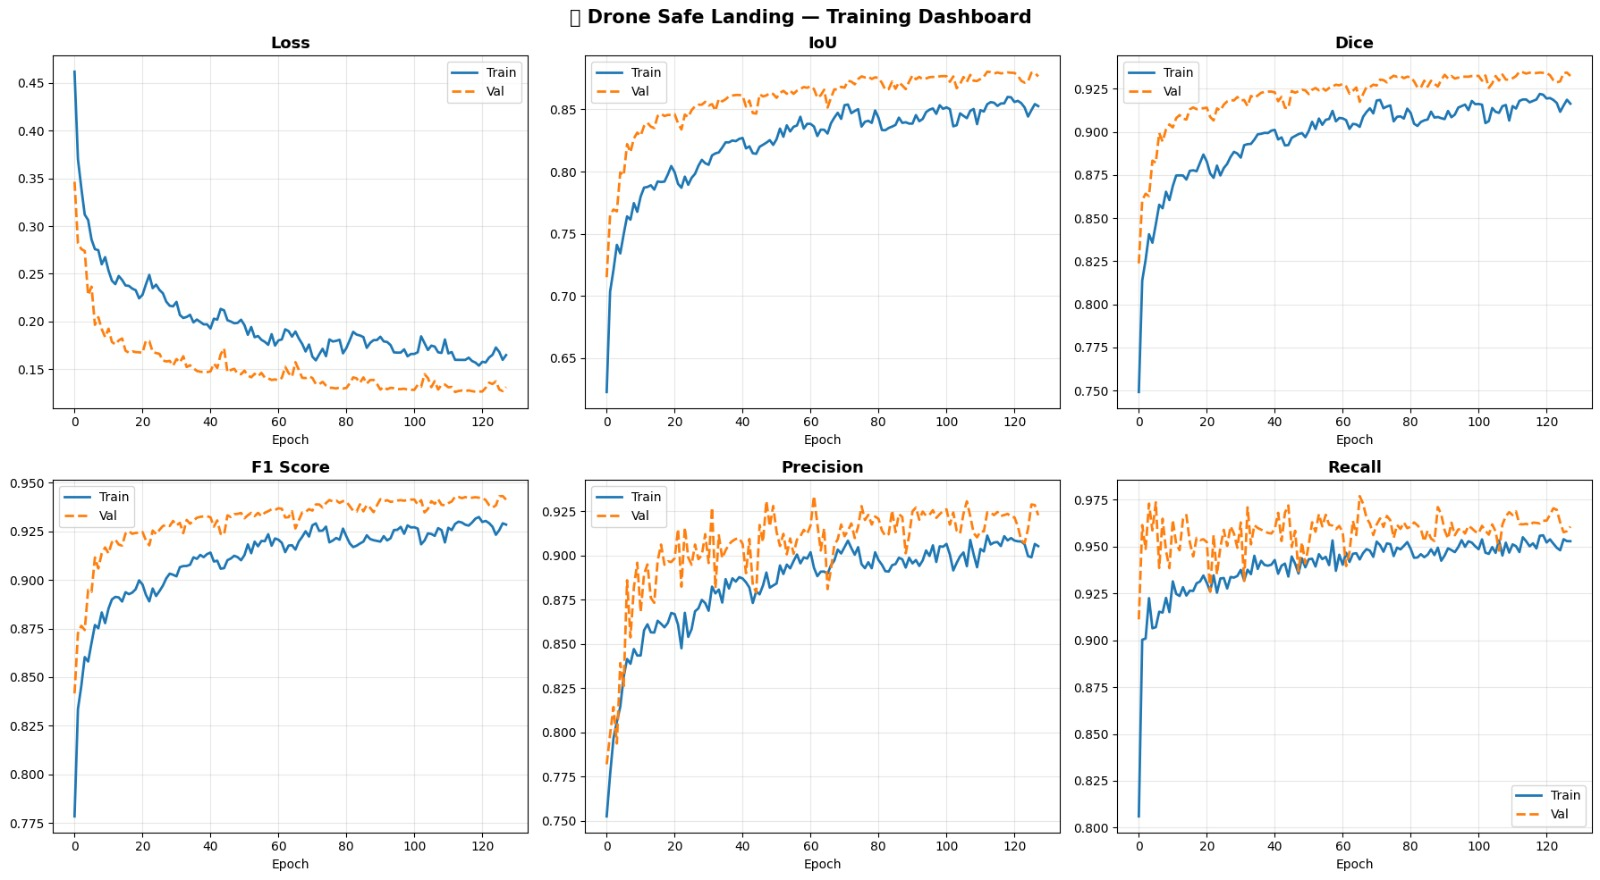
\includegraphics[width=0.75\textwidth,keepaspectratio]{diagramme.jpeg}
  \caption{Courbes d'évolution de la perte (Loss), de l'IoU, du Dice Score, du F1-Score, de la Precision et du Recall en entraînement et validation.}
  \label{fig:training-curves}
\end{figure}

Les journaux d'entraînement (logs console) confirment le bon déroulement du processus, avec la sauvegarde automatique des checkpoints dès qu'une amélioration de la perte de validation est détectée (figure~\ref{fig:training-logs}). Cet extrait montre en particulier les métriques intermédiaires obtenues entre les époques 98 et 101, illustrant la phase de stabilisation progressive. L'entraînement s'est ensuite poursuivi au-delà de cette phase jusqu'à atteindre les performances optimales du meilleur modèle sauvegardé à l'époque 113, avant le déclenchement final de l'arrêt anticipé (Early Stopping) après stabilisation à l'époque 128.

\begin{figure}[!ht]
  \centering
  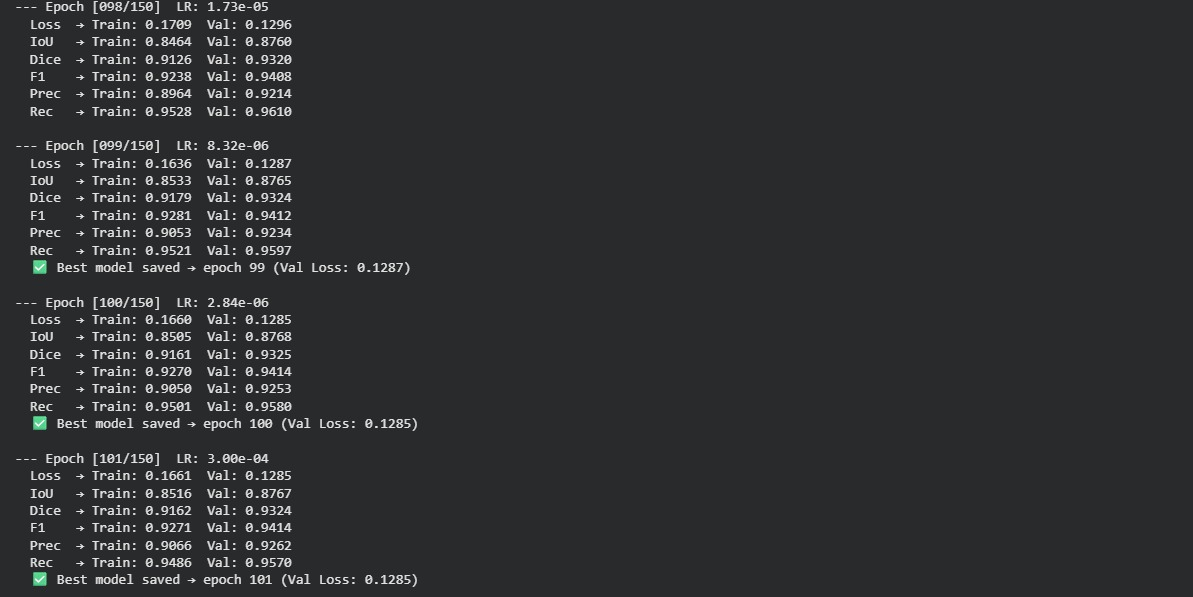
\includegraphics[width=0.65\textwidth,keepaspectratio]{train_Epochs.jpeg}
  \caption{Extrait des journaux d'entraînement (logs console) montrant l'évolution des métriques (Loss, IoU, Dice, F1, Precision, Recall) entre les époques 98 et 101, avec sauvegarde automatique du meilleur modèle.}
  \label{fig:training-logs}
\end{figure}

\textbf{\textcolor{red}{Note :}} Les courbes de validation restent globalement proches des courbes d'entraînement tout au long du processus — la perte de validation est même légèrement inférieure à la perte d'entraînement sur les dernières époques —, ce qui n'indique pas de surapprentissage marqué. La Data Augmentation et la régularisation (Weight Decay) semblent avoir rempli leur rôle.

Au-delà des scores globaux, la validation du système repose sur une inspection visuelle directe des prédictions du modèle sur des scènes réelles, présentée ci-après.

\section{Résultats visuels}
\label{sec:resultats-visuels}

L'inspection qualitative sur un échantillon varié de scènes de test (figure~\ref{fig:predictions-comparison}) confirme la précision spatiale du modèle. Les quatre exemples présentés illustrent la capacité du réseau à segmenter correctement les surfaces d'atterrissage praticables tout en isolant les piétons, véhicules et autres obstacles critiques, avec des scores d'intersection sur union (IoU) individuels élevés.

\begin{figure}[!hb]
  \centering
  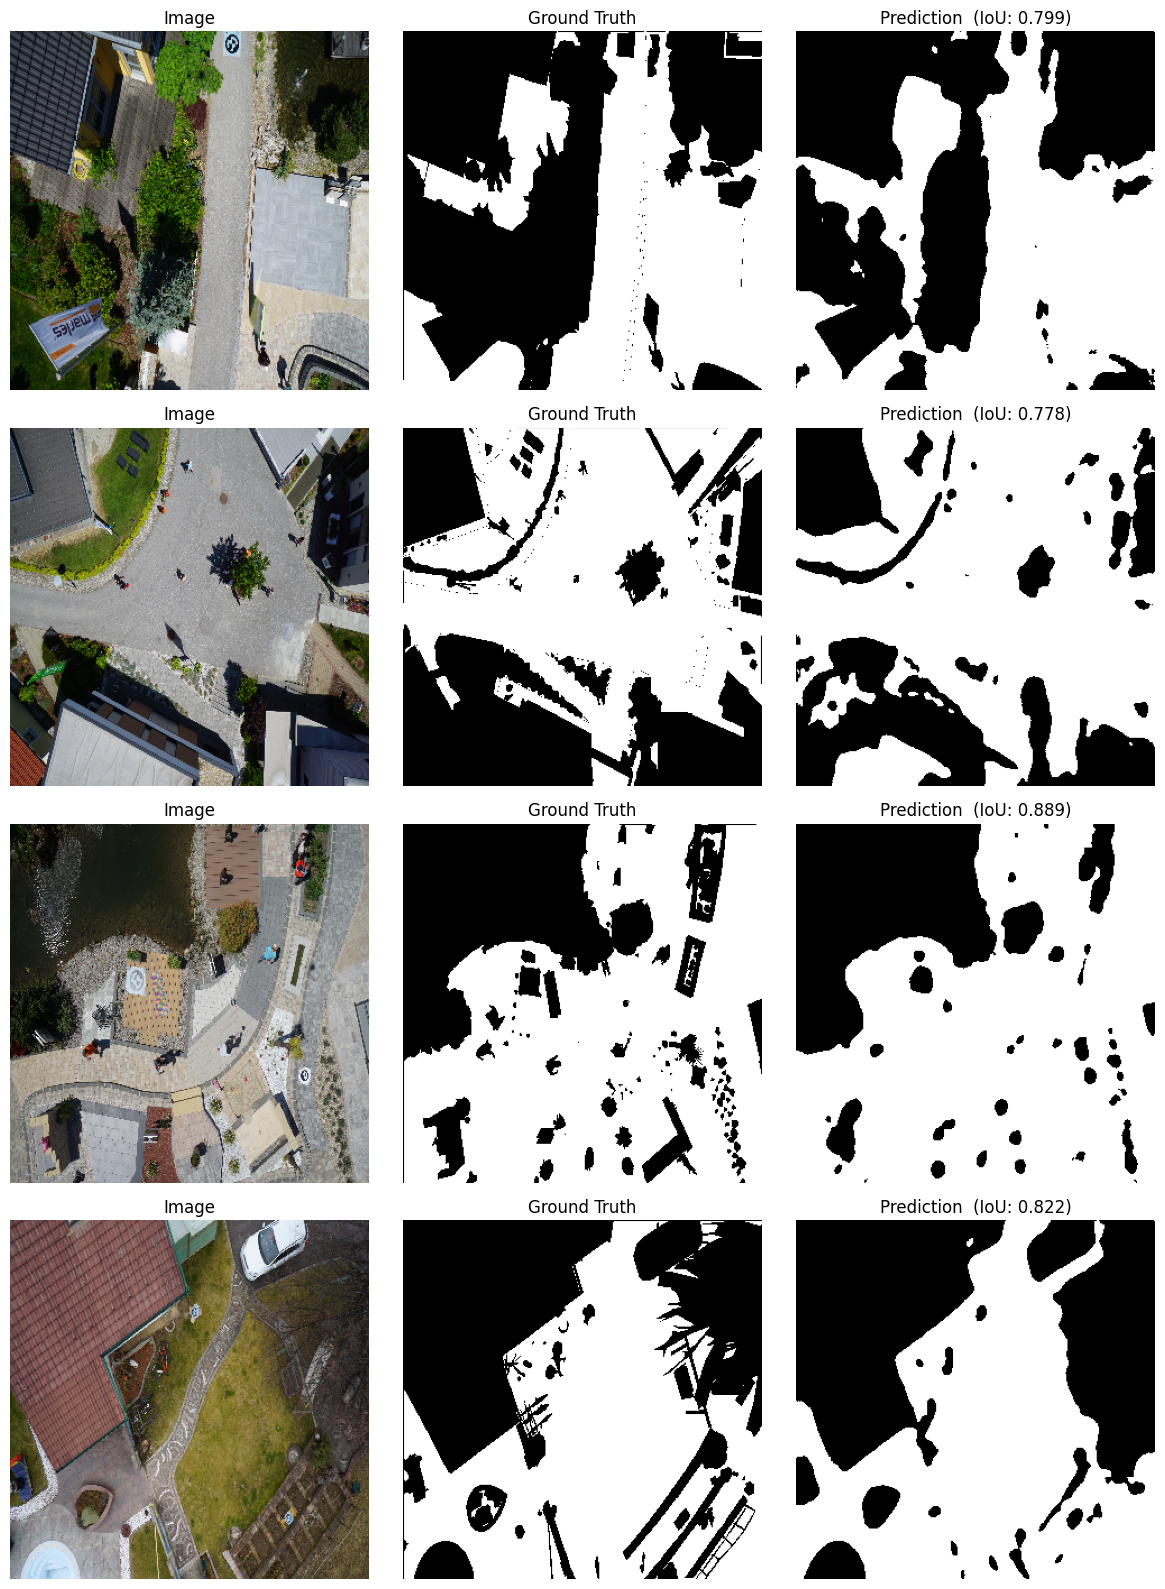
\includegraphics[width=0.7\textwidth,keepaspectratio]{slide14_resultats_visuels.png}
  \caption{Comparaison qualitative sur le dataset de test pour quatre exemples caractéristiques : image d'entrée, vérité terrain (Ground Truth) et masque de prédiction sémantique avec l'indice de Jaccard (IoU) obtenu pour chaque scène.}
  \label{fig:predictions-comparison}
\end{figure}

Ce comportement illustre le fonctionnement attendu du pipeline de décision : la conversion du masque sémantique en carte binaire exploitable identifie correctement les obstacles ponctuels (personnes, objets) tout en conservant de larges surfaces continues pour l'atterrissage.

Afin de situer la performance de notre modèle sémantique par rapport aux standards actuels, nous le comparons avec les architectures de référence de la littérature.

\section{Comparaison avec les architectures de la littérature}
\label{sec:comparaison}

Le choix de l'architecture U-Net + EfficientNet-B0 a été justifié au chapitre~\ref{chap:dataset} par une comparaison qualitative avec les approches les plus utilisées en segmentation sémantique. FCN offre un coût de calcul faible mais une reconstruction des détails plus limitée ; DeepLabV3 et SegFormer atteignent une précision potentiellement supérieure au prix d'un coût mémoire et d'un temps d'inférence incompatibles avec les contraintes Edge AI.

Les résultats obtenus (IoU 0.8803, Dice 0.9349) confirment qu'une architecture plus légère, correctement optimisée, peut atteindre un niveau de performance élevé tout en restant compatible avec un déploiement embarqué. Pour finaliser cette évaluation, il convient de dresser un bilan critique des forces de notre approche ainsi que des limites qui tracent les perspectives futures.

\section{Discussion, forces et limites}
\label{sec:discussion}

Les résultats obtenus valident l'approche retenue : un IoU de validation de \textbf{0.8803}, un Dice Score de \textbf{0.9349}, une précision de \textbf{0.9305}, un rappel de \textbf{0.9393} et un F1-Score global de \textbf{0.9349}. Ces niveaux de performance, classés comme \textit{excellents} selon les seuils établis, démontrent la robustesse du réseau tant pour la détection fiable des zones praticables que pour la non-omission d'obstacles critiques, le tout avec une convergence stable et sans surapprentissage marqué.

Ces résultats doivent néanmoins être interprétés avec les réserves suivantes :
\begin{itemize}[leftmargin=1.8em, itemsep=4pt]
  \item[\textcolor{ENIADOrange}{\ding{118}}] Le dataset reste limité (400 images), ce qui restreint la diversité des scènes réellement couvertes ;
  \item[\textcolor{ENIADOrange}{\ding{118}}] Les métriques sont mesurées hors ligne, et non lors d'une exécution embarquée en conditions réelles ;
  \item[\textcolor{ENIADOrange}{\ding{118}}] La comparaison avec d'autres architectures reste théorique faute de benchmark empirique direct.
\end{itemize}

\vspace{1.5em}
\textbf{Conclusion}

En conclusion, ce quatrième et dernier chapitre a permis de valider expérimentalement les performances du système développé en obtenant des scores élevés en validation (IoU de 0.8803 et Dice Score de 0.9349) et en confirmant qualitativement la fiabilité de la Distance Transform. Les discussions critiques ont également tracé la voie pour de futures améliorations matérielles et de déploiement réel. Ce bilan expérimental venant clore notre étude technique, la conclusion générale suivante synthétisera l'ensemble de nos contributions académiques et ouvrira sur les perspectives industrielles à long terme de ce projet.
\clearpage

% ============================================================
%  CONCLUSION GÉNÉRALE
% ============================================================
\chapter*{Conclusion Générale}
\addcontentsline{toc}{chapter}{Conclusion Générale}
\markboth{Conclusion Générale}{Conclusion Générale}

Ce projet avait pour ambition de répondre à une question concrète : est-il possible, à partir d'une simple image aérienne, de doter un drone autonome de la capacité à identifier automatiquement une zone d'atterrissage sécurisée en situation d'urgence ? Les travaux réalisés montrent que la réponse est \textbf{oui} — sous réserve des conditions et limites clairement identifiées tout au long de ce rapport.

En combinant segmentation sémantique profonde, transfert d'apprentissage et optimisations orientées Edge AI, le système développé atteint un \textbf{Val IoU de 0.8803} et un \textbf{Val Dice Score de 0.9349} sur le Graz Semantic Drone Dataset (avec une précision de \textbf{0.9305} et un rappel de \textbf{0.9393} au meilleur modèle), des performances classées excellentes selon les seuils retenus.

L'évaluation finale du système met en évidence un bilan positif au regard des objectifs fixés. L'objectif d'identification des zones sûres d'atterrissage et la segmentation multiclasses des 24 catégories sémantiques sont pleinement atteints, grâce à la précision spatiale fine apportée par l'architecture Attention U-Net combinée à la data augmentation. En revanche, la détection des obstacles est jugée partiellement atteinte, car si le modèle segmente fidèlement les menaces de grande envergure (bâtiments, routes encombrées), des limitations persistent sur les petits obstacles ponctuels (personnes isolées, poteaux fins) en raison du sous-échantillonnage de l'encodeur.

Sur le plan de l'intégration, la robustesse environnementale est globalement atteinte grâce à la diversité des scènes du Graz Semantic Drone Dataset et à l'entraînement sous conditions d'augmentation variées. La compatibilité avec les plateformes Edge AI est quant à elle prometteuse, démontrée par la légèreté de l'encodeur EfficientNet-B0 et la portabilité offerte par le format ONNX. Toutefois, le traitement temps réel complet reste à améliorer ; bien que l'inférence théorique réponde aux exigences, une validation physique et matérielle embarquée sur carte Jetson Orin reste nécessaire pour confirmer les temps de réponse de la boucle fermée de contrôle.

\vspace{0.6em}
\textbf{Limites identifiées :} Le volume du dataset reste limité (400 images), restreignant la diversité des scènes couvertes. La validation embarquée réelle (latence, FPS, consommation) reste à conduire. La variabilité des conditions (nuit, pluie, forte luminosité) constitue un angle mort potentiel.

\vspace{0.6em}
\textbf{Perspectives :} À court terme, l'export du modèle en ONNX/TensorRT et la validation sur processeur embarqué (Jetson Nano). À moyen terme, l'enrichissement du dataset et l'amélioration de la détection des petits objets. À long terme, la fusion multimodale capteurs/vision, l'exploration des Vision Transformers et un agent de Reinforcement Learning pour une stratégie d'atterrissage dynamique.

\vspace{0.6em}
En définitive, ce projet démontre qu'il est possible, avec des ressources limitées et un dataset de taille modeste, de construire un système de segmentation sémantique performant et orienté vers l'embarqué — une contribution concrète vers la nouvelle génération de drones autonomes capables de \textbf{percevoir, comprendre et décider} en toute sécurité.

\clearpage

% ============================================================
%  ANNEXE UNIQUE : EXTRAITS DE CODE SOURCE
% ============================================================
\appendix

\chapter{Extraits de code source}
\label{ann:code}

Cette annexe contient les extraits les plus significatifs du code d'entraînement, de préparation des données et de guidage du modèle développé dans ce projet.

\subsection{Configuration et Hyperparamètres}

L'extrait suivant présente les hyperparamètres et la configuration globale utilisés pour initialiser l'entraînement (définis dans la cellule 21 du notebook).

\begin{lstlisting}[language=Python, caption={Hyperparamètres globaux d'entraînement.}]
# -- Image
IMG_SIZE    = 320
IN_CHANNELS = 3

# -- Training
EPOCHS         = 150
BATCH_SIZE     = 8
LEARNING_RATE  = 3e-4
WEIGHT_DECAY   = 1e-4
MAX_GRAD_NORM  = 1.0

# -- Scheduler & early stop
PATIENCE_ES    = 15
PATIENCE_LR    = 5

# -- ImageNet stats (correct for pretrained encoders)
IMAGENET_MEAN = (0.485, 0.456, 0.406)
IMAGENET_STD  = (0.229, 0.224, 0.225)
\end{lstlisting}

\subsection{Dataset et augmentation de données}
\label{sec:code-dataset-augmentation}

L'implémentation de la classe personnalisée PyTorch \texttt{DroneDataset} et la chaîne d'augmentation de données basée sur Albumentations (cellules 27 et 29 du notebook).

\begin{lstlisting}[language=Python, caption={Pipeline d'augmentation et classe de chargement des données.}]
# Pipeline d'augmentation pour l'entraînement
train_transform = A.Compose([
    A.Resize(IMG_SIZE, IMG_SIZE),
    A.HorizontalFlip(p=0.5),
    A.VerticalFlip(p=0.3),
    A.RandomRotate90(p=0.5),
    A.ShiftScaleRotate(
        shift_limit=0.1, scale_limit=0.2, rotate_limit=30,
        border_mode=cv2.BORDER_REFLECT_101, p=0.7
    ),
    A.Perspective(scale=(0.04, 0.08), p=0.3),
    A.RandomBrightnessContrast(brightness_limit=0.3, contrast_limit=0.3, p=0.6),
    A.CoarseDropout(
        max_holes=8, max_height=32, max_width=32,
        min_holes=1, fill_value=0, mask_fill_value=0, p=0.3
    ),
    A.Normalize(mean=IMAGENET_MEAN, std=IMAGENET_STD),
    ToTensorV2(),
])

class DroneDataset(Dataset):
    """Binary segmentation: SAFE (1) vs UNSAFE (0) landing zones."""
    SAFE_CLASSES = [1, 3] # paved-area (1), grass (3)

    def __init__(self, img_list, mask_list, img_dir, mask_dir, transform=None):
        self.img_list  = img_list
        self.mask_list = mask_list
        self.img_dir   = img_dir
        self.mask_dir  = mask_dir
        self.transform = transform

    def __len__(self):
        return len(self.img_list)

    def __getitem__(self, idx):
        img_path  = os.path.join(self.img_dir,  self.img_list[idx])
        mask_path = os.path.join(self.mask_dir, self.mask_list[idx])

        image = cv2.imread(img_path)
        image = cv2.cvtColor(image, cv2.COLOR_BGR2RGB)
        mask = cv2.imread(mask_path, cv2.IMREAD_GRAYSCALE)

        # Binarisation: 1.0 = SAFE, 0.0 = UNSAFE
        mask = np.isin(mask, self.SAFE_CLASSES).astype(np.float32)

        if self.transform:
            augmented = self.transform(image=image, mask=mask)
            image = augmented["image"]
            mask  = augmented["mask"]

        return image, mask.unsqueeze(0)
\end{lstlisting}

\subsection{Architecture du modèle et fonction de coût}

Le code ci-dessous montre la définition du modèle via la bibliothèque \texttt{segmentation\_models\_pytorch} et la fonction de coût hybride combinant la BCE logarithmique et la Tversky Loss.

\begin{lstlisting}[language=Python, caption={Définition du modèle U-Net et de la fonction de coût.}]
# Modèle U-Net avec encodeur EfficientNet-B0 pré-entraîné
model = smp.Unet(
    encoder_name    = "efficientnet-b0",
    encoder_weights = "imagenet",
    in_channels     = IN_CHANNELS,
    classes         = 1,
    activation      = None,
    decoder_use_batchnorm = True,
)
model = model.to(DEVICE)

# Definition des fonctions de cout
bce_loss = nn.BCEWithLogitsLoss()
tversky_loss = smp.losses.TverskyLoss(
    mode="binary", alpha=0.3, beta=0.7, smooth=1e-6
)

def loss_fn(pred, target):
    return 0.5 * bce_loss(pred, target) + 0.5 * tversky_loss(pred, target)
\end{lstlisting}

\subsection{Contrôleur de guidage et machine d'états}
\label{sec:code-guidage-machine}

Ces classes et fonctions implémentent le pipeline d'évitement géométrique et la logique de pilotage de haut niveau qui traite la prédiction du modèle.

\begin{lstlisting}[language=Python, caption={Algorithme de guidage géométrique et machine d'états de vol.}]
# Guidance Controller
def guidance_controller(landing_x, landing_y, image_width, image_height, tolerance=10):
    center_x = image_width // 2
    center_y = image_height // 2

    # Calcul de l'erreur en pixels
    dx = landing_x - center_x
    dy = landing_y - center_y

    distance = math.sqrt(dx**2 + dy**2)
    heading = math.degrees(math.atan2(dy, dx))

    # Logique de guidage horizontal et vertical
    horizontal = "MOVE RIGHT" if dx > tolerance else ("MOVE LEFT" if dx < -tolerance else "HOLD")
    vertical = "MOVE BACKWARD" if dy > tolerance else ("MOVE FORWARD" if dy < -tolerance else "HOLD")
    centered = abs(dx) <= tolerance and abs(dy) <= tolerance

    return {
        "landing_x": landing_x, "landing_y": landing_y,
        "center_x": center_x, "center_y": center_y,
        "dx": dx, "dy": dy, "distance": distance, "heading": heading,
        "horizontal": horizontal, "vertical": vertical, "centered": centered
    }

# Machine d'états de vol
class FlightState(Enum):
    SEARCHING = "SEARCHING"
    GUIDING = "GUIDING"
    LANDING = "LANDING"

class FlightStateMachine:
    def __init__(self):
        self.state = FlightState.SEARCHING

    def update(self, landing_allowed, centered):
        if self.state == FlightState.SEARCHING:
            if landing_allowed:
                self.state = FlightState.GUIDING
        elif self.state == FlightState.GUIDING:
            if not landing_allowed:
                self.state = FlightState.SEARCHING
            elif centered:
                self.state = FlightState.LANDING
        elif self.state == FlightState.LANDING:
            if not landing_allowed:
                self.state = FlightState.SEARCHING
        return self.state
\end{lstlisting}

\clearpage


\bibliographystyle{unsrtnat}
\bibliography{references}

\end{document}
